% sonifold_jmaa.tex
% Rewritten for Journal of Mathematics and the Arts

\documentclass[]{interact}

\usepackage{graphicx}
\usepackage{epstopdf}
\usepackage[caption=false]{subfig}
\usepackage{amsmath,amssymb}
\usepackage{array} % better column types (e.g., raggedright p{..} columns)

% --- Float placement helpers (keep figures near where they are mentioned) ---
\usepackage{float} % provides the [H] specifier if you ever need to force placement
\usepackage[section]{placeins} % automatically inserts \FloatBarrier at each \section

\usepackage[longnamesfirst,sort]{natbib}
\bibpunct[, ]{(}{)}{;}{a}{,}{,}
\renewcommand\bibfont{\fontsize{10}{12}\selectfont}
\usepackage{tikz}
\usepackage{url}
\usepackage{hyperref}
\usetikzlibrary{shapes.geometric,arrows.meta,positioning}

\theoremstyle{plain}
\newtheorem{theorem}{Theorem}[section]

\theoremstyle{definition}
\newtheorem{definition}[theorem]{Definition}
\newtheorem{example}[theorem]{Example}

\theoremstyle{remark}
\newtheorem{remark}{Remark}
\newtheorem{conjecture}[theorem]{Conjecture}

\begin{document}

\articletype{Research Article}

\title{Sonifold: Audio-Driven Nodal Surfaces on 3D Meshes}

\author{
  Joonhyung Bae \\
  Graduate School of Culture Technology \\
  KAIST (Korea Advanced Institute of Science and Technology) \\
  Daejeon, South Korea \\
  \texttt{jh.bae@kaist.ac.kr} \\
ORCID: \href{https://orcid.org/0000-0001-5933-4302}{0000-0001-5933-4302}
}

\maketitle

%% ====================================================================
%% ABSTRACT
%% ====================================================================
\begin{abstract}
In 1787 Ernst Chladni scattered sand on vibrating plates and revealed the hidden geometry of sound. We extend this idea to arbitrary three-dimensional shapes: given a triangle mesh---a sphere, a torus, a double torus---we define a scalar field from audio input using the eigenfunctions of the Laplace--Beltrami operator and extract its nodal surface, the locus where the field vanishes. Because the eigenfunctions depend on the intrinsic geometry of the underlying shape, the same audio signal produces visually distinct nodal patterns on different meshes; in this sense, the shape acts as a \emph{geometry-dependent spectral filter}.

We describe a mathematical framework connecting the short-time Fourier transform of an audio signal to the spectral decomposition on a manifold, present three coefficient-mapping strategies, and introduce topological and symmetry indices ($\beta_0$, $A_{\mathrm{ratio}}$, $S$) that quantify the visual complexity of the resulting nodal pattern. An exploration across nine meshes and seven audio stimuli reveals that spectral characteristics of the shape --eigenvalue density, spectral gap, and symmetry---systematically govern the complexity of the nodal pattern; a genus sequence shows that this dependence is non-monotonic, and frame-by-frame time series show that nodal topology tracks audio dynamics. We discuss the resulting \emph{visual vocabulary} and provide an interactive web application.
\end{abstract}

\begin{keywords}
nodal surfaces; Chladni patterns; Laplace--Beltrami eigenfunctions;
spectral geometry; music visualization; generative art; mathematical art;
topology; audio-visual mapping
\end{keywords}


%% ====================================================================
\section{Introduction}
\label{sec:intro}
%% ====================================================================

In the late 18th century, the physicist and musician Ernst Chladni drew a violin bow along the edge of a metal plate dusted with fine sand and watched the sand collect along lines where the plate did not vibrate \citep{chladni1787entdeckungen,chladni1830}. These \emph{nodal lines}, the zero-displacement curves, revealed the vibrational character of the plate in a single striking image, and the patterns became icons at the intersection of physics and aesthetics.

The mathematical theory arrived in stages. Weyl's asymptotic law related the distribution of eigenvalues to the volume and dimension of the vibrating domain \citep{jrgens1964}; Courant's nodal-domain theorem placed an upper bound on the number of connected regions between nodal lines \citep{courant1923allgemeiner}; and in 1966, Mark Kac asked \emph{``Can one hear the shape of a drum?''} \citep{kac1966}, crystallizing the deep connection between geometry and spectrum. The answer, as \citet{gordon1992} showed, is ``not always,'' but the question continues to inspire new work in spectral geometry.

In this article, we carry Chladni's idea into three dimensions and into the realm of digital audio. Rather than vibrating a physical plate, we take a three-dimensional mesh---sphere, torus, double torus, and others---and use the eigenfunctions of the \emph{Laplace--Beltrami} (LB) operator on that mesh as analogs of Chladni's vibrational modes. The audio input is analyzed by the short-time Fourier transform (STFT), and the resulting frequency coefficients are mapped onto the LB eigenfunction coefficients to define a scalar field on the surface. The zero-level set of this field is our three-dimensional generalization of the Chladni figure.

The central observation is that the same audio produces visually different nodal patterns in different shapes. A pure tone yields a clean banded structure on a sphere, an interlocking lattice on a torus, and a fragmented mosaic on a double torus. Geometry acts as a \emph{spectral filter}: it selects, distorts, and transforms audio information into a shape-specific visual form. This filtering is a direct consequence of the fact that the eigenfunctions~$\phi_k$ and the eigenvalues~$\lambda_k$ of the LB operator depend on the geometry of the manifold.

Our contributions are as follows.
\begin{enumerate}
\item A generative framework in which the choice of 3D shape becomes a controllable parameter --analogous to the choice of tuning system in music or tiling rule in pattern design---that systematically transforms audio input into geometry-dependent visual patterns. The framework couples the STFT of an audio signal with the LB eigenbasis of a mesh through an explicit coefficient mapping. The mathematical novelty lies not in the individual components, which are well established, but in their systematic coupling and in the resulting \emph{shape-as-filter} principle: spectral properties of the mesh (eigenvalue density, spectral gap, symmetry) predict the topological complexity of the nodal pattern in a consistent and interpretable way. The mathematical exposition emphasizes geometric intuition for a dual mathematical--artistic readership (Section~\ref{sec:background}).

\item Three mapping strategies (direct, mel-weighted, energy-weighted) from audio coefficients to eigenfunction coefficients, together with topological and symmetry indices ($\beta_0$, $A_{\mathrm{ratio}}$,~$S$) for characterizing the resulting patterns (Section~\ref{sec:method}).

\item A systematic exploration of the \emph{visual vocabulary} produced by nine meshes and seven audio stimuli, including a random-baseline comparison establishing that audio-driven patterns differ from random excitation (Section~\ref{sec:random_baseline}); quantitative analysis relating spectral shape properties (spectral gap, eigenvalue density, symmetry) to visual complexity (Section~\ref{sec:quantitative}); and shape-sequencing studies illustrating compositional use (Section~\ref{sec:sequencing}).

\item A genus sequence (genus~0 through~6) revealing a non-monotonic relationship between topology and nodal complexity, and the introduction of \emph{spectral entropy} as a unifying descriptor that accounts for this non-monotonicity where genus alone cannot (Sections~\ref{sec:genus}--\ref{sec:spectral_entropy}). Frame-by-frame time series further demonstrate that nodal topology tracks audio dynamics (Section~\ref{sec:temporal}).

\item A discussion of how shape selection functions as a generative parameter and what visual qualities each class of shape affords (Section~\ref{sec:artistic}), together with an interactive web application for real-time exploration (Section~\ref{sec:interactive}).
\end{enumerate}

We situate this work at the intersection of spectral geometry, audio analysis, and generative art. The paper is addressed to readers from both mathematical and artistic backgrounds; we have tried to keep the mathematical exposition self-contained and to accompany formal statements with visual examples and geometric intuition. For the practice-oriented reader, the key takeaway is that \emph{choosing a shape is choosing a visual filter}: the mathematical framework explains why this is so and what each shape affords. An interactive web application for real-time exploration is provided as supplementary material (Section~\ref{sec:interactive}).

\begin{figure}[!htbp]
\centering
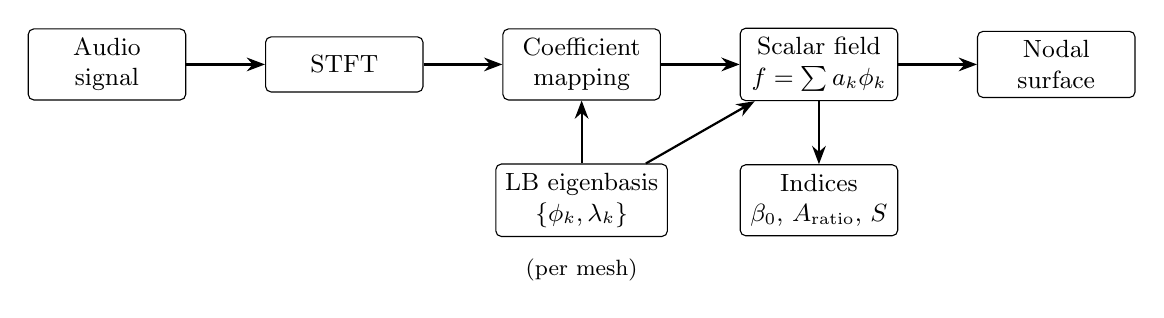
\begin{tikzpicture}[node distance=1.0cm, every node/.style={font=\small},
  block/.style={rectangle, draw, rounded corners=2pt,
                minimum width=2.0cm, minimum height=0.7cm, align=center},
  arrow/.style={-Stealth, thick}]
  \node[block] (audio) {Audio\\signal};
  \node[block, right=of audio] (stft) {STFT};
  \node[block, right=of stft] (map) {Coefficient\\mapping};
  \node[block, right=of map] (field) {Scalar field\\$f = \sum a_k \phi_k$};
  \node[block, right=of field] (nodal) {Nodal\\surface};
  \node[block, below=0.8cm of map] (eigen) {LB eigenbasis\\$\{\phi_k, \lambda_k\}$};
  \node[font=\footnotesize, below=0.15cm of eigen] (eigenlabel) {(per mesh)};
  \node[block, below=0.8cm of field] (indices) {Indices\\$\beta_0$, $A_{\mathrm{ratio}}$, $S$};
  \draw[arrow] (audio) -- (stft);
  \draw[arrow] (stft) -- (map);
  \draw[arrow] (map) -- (field);
  \draw[arrow] (field) -- (nodal);
  \draw[arrow] (eigen) -- (map);
  \draw[arrow] (eigen) -- (field);
  \draw[arrow] (field) -- (indices);
\end{tikzpicture}
\caption{Overview of the audio-to-nodal-surface pipeline. Audio is analysed by the STFT; frequency coefficients are mapped to eigenfunction coefficients via the Laplace--Beltrami eigenbasis of a chosen 3D mesh; the scalar field~$f$ and its nodal surface are computed; and topological and symmetry indices characterise the pattern. The eigenbasis (bottom left) is what makes the mapping geometry-dependent: it defines the coefficient target and, through~$\phi_k$, the resulting field.}
\label{fig:pipeline}
\end{figure}

%% ====================================================================
\section{Related work}
\label{sec:related}
%% ====================================================================

\subsection{Chladni figures, cymatics, and spectral geometry}

The study of vibrating plates and their nodal patterns has a rich history, from Chladni's original experiments \citep{chladni1787entdeckungen,chladni1830} through the mathematical theories of Germain, Kirchhoff, and Rayleigh. \citet{jenny2001} extended the visual repertoire by documenting vibration patterns in fluids and on membranes, coining the term \emph{cymatics}; recent work has revisited Chladni figures at the nanoscale \citep{dorrestijn2007chladni}.

The spectrum of the Laplace--Beltrami operator on a Riemannian manifold encodes geometric information about the manifold. Weyl's law \citep{jrgens1964} describes the asymptotic growth of eigenvalues; Courant's theorem \citep{courant1923allgemeiner} limits the number of nodal domains; and Kac's question \citep{kac1966}, answered negatively by \citet{gordon1992}, continues to motivate spectral geometry. For surveys of geometric properties of eigenfunctions, see \citet{jakobson2001}; for topological properties of nodal domains, see \citet{band2016}. In computational geometry, \citet{reuter2006laplace} introduced the LB spectrum as a ``Shape-DNA'' descriptor, and \citet{vallet2008} developed manifold-harmonics methods for mesh processing. We build on the computational infrastructure of manifold harmonics but, unlike physical cymatics or shape-descriptor applications, use a pre-computed eigenbasis to construct scalar fields from external audio input, treating the shape as a fixed geometric filter rather than simulating vibrations or characterizing shape alone.

\subsection{Mathematics of music and audio--visual mapping}

The mathematical analysis of musical sound has deep roots in Fourier theory and its extensions. \citet{benson2006} and \citet{loy2007} provide comprehensive treatments; \citet{sethares1998} explores the relationship between tuning, timbre, and spectral content. In a geometric direction, \citet{tymoczko2006} and \citet{callender2008} model chord progressions as paths in geometric spaces, and \citet{cohn2012} develop a neo-Riemannian theory of triadic harmony. In this journal, \citet{trevio2022} connects tilings and meter to generate music from aperiodic substitution systems. Our work connects to this tradition by linking \emph{the audio spectrum}, \emph{the 3D shape}, and \emph{the visualization} of the nodal surface: the audio spectral content is mapped onto the eigenbasis of a manifold to produce geometry-dependent nodal patterns.

\subsection{Sound visualization and generative mathematical art}

\citet{lima2022} review music-visualization techniques from waveform displays to immersive 3D representations. Systems such as CymaSense \citep{mcgowan2017} map audio features to visual parameters in real time. The mapping of parameters \citep{grond2011parameter,hermann2011sonification} and the auditory presentation research have developed systematic frameworks; yet the mapping of audio to visuals typically remains ad hoc, driven by amplitude envelopes or spectral centroids rather than by a basis tied to the geometry of the display surface. In contrast to these systems, the present framework mediates the mapping through the LB eigenbasis of a specific mesh, so the geometry explicitly and predictably filters the result.

The use of mathematical structures as a basis for art has a long history, from geometric art surveyed by \citet{ghyka1946} to Escher's symmetry explorations \citep{schattschneider2010mathematical} to mathematically informed computational art \citep{feijs2019}. The Bridges conference and this journal have highlighted mathematically grounded approaches to art \citep{harriss2022,goldstine2017}, including special issues on mathematical illustration and fiber arts \citep{belcastro2023}. Our framework offers a new generative mechanism --audio-driven nodal surfaces---that is mathematically grounded and open-ended.

%% ====================================================================
\section{Mathematical background}
\label{sec:background}
%% ====================================================================

This section presents the mathematical ideas underlying the audio-to-nodal-surface mapping. We aim for geometric intuition alongside formal statements, using the sphere as a running example.

\subsection{The Laplace--Beltrami operator and its eigenfunctions}
\label{sec:lb}

On a smooth closed surface~$M$ embedded in~$\mathbb{R}^3$, the \emph{Laplace--Beltrami} (LB) operator~$\Delta_M$ generalizes the Laplacian~$\nabla^2$ from flat space to curved surfaces \citep{rosenberg1997laplacian}. Informally, $\Delta_M f(p)$ measures how the value of~$f$ at~$p$ deviates from its average in a small neighborhood of~$p$; on a curved surface the curvature modifies the averaging, so the operator ``knows'' the geometry.

The eigenfunctions~$\phi_k$ and eigenvalues~$\lambda_k$ satisfy
\begin{equation}
\label{eq:eigenvalue}
-\Delta_M \phi_k = \lambda_k \, \phi_k,
\qquad 0 = \lambda_0 \le \lambda_1 \le \lambda_2 \le \cdots,
\end{equation}
where $\phi_0$ is constant and the remaining eigenfunctions are orthonormal with respect to the inner product of the surface-area. These eigenfunctions are the \emph{natural vibration modes} of the surface: $\phi_k$ represents a pattern that, were the surface a drum or a bell, would vibrate at a frequency proportional to~$\sqrt{\lambda_k}$.

\begin{example}[Sphere]
In the unit sphere~$S^2$, the eigenfunctions are the \emph{spherical harmonics}~$Y_\ell^m$ with eigenvalues $\lambda = \ell(\ell+1)$, $\ell = 0,1,2,\ldots$ and $-\ell \le m \le \ell$. For $\ell=1$ there are three eigenfunctions with a single nodal circle each; for $\ell=2$, five eigenfunctions with more complex nodal curves (Figure~\ref{fig:spherical}). Note the high multiplicity: $\ell(\ell+1)$ has multiplicity~$2\ell+1$, a consequence of the sphere's rotational symmetry.
\end{example}

\begin{figure}[!htbp]
\centering
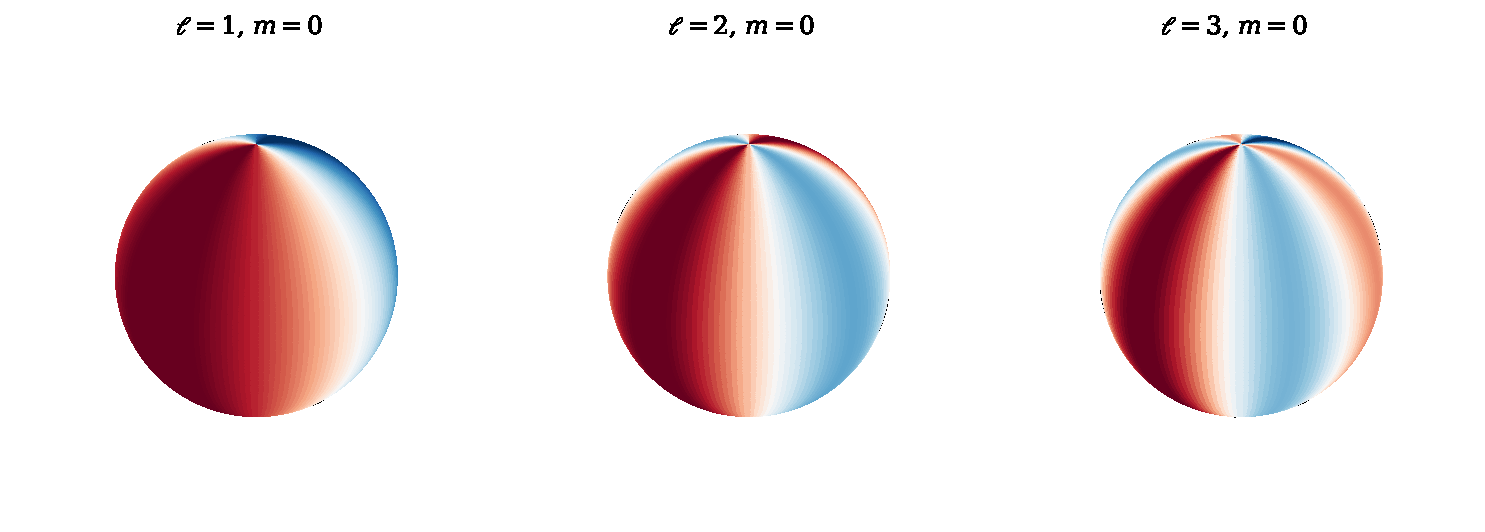
\includegraphics[width=0.85\linewidth]{figures/fig8_spherical_harmonics.pdf}
\caption{Low-order spherical harmonics on the unit sphere, with nodal lines shown in black. For $\ell=1$ each eigenfunction has a single nodal circle; for $\ell=2$ and~$\ell=3$ the nodal curves become progressively more complex. On other shapes the eigenfunctions and their nodal geometry differ.}
\label{fig:spherical}
\end{figure}

A torus, having different geometry and a non-trivial fundamental group, has a different spectrum and different eigenfunctions; the same coefficients mapped to these different eigenfunctions yield different nodal patterns.

\subsection{Nodal sets and nodal domains}
\label{sec:nodal}

Given a function $f\colon M \to \mathbb{R}$, the \emph{nodal set} is $N(f) = \{ p \in M : f(p) = 0 \}$. On a two-dimensional surface, the nodal set of a single eigenfunction~$\phi_k$ is generically a collection of smooth curves dividing~$M$ into \emph{nodal domains}, connected regions of constant sign. (Throughout this paper, we use \emph{the nodal surface} loosely in the title and in informal discussion to evoke the three-dimensional embedding of the mesh; the precise object is the nodal set, which on a two-dimensional surface is generically one-dimensional.) Courant's theorem \citep{courant1923allgemeiner} states that $\phi_k$ has at most $k+1$ nodal domains.

For a linear combination $f = \sum_k a_k \phi_k$, the nodal set can be considerably more complex than any single eigenfunction: curves can intersect, form closed loops, or create intricate networks. This complexity makes audio-driven combinations visually rich.

\subsection{Weyl's law and eigenvalue density}
\label{sec:weyl}

Weyl's asymptotic law \citep{jrgens1964} states that for a two-dimensional surface~$M$ of area~$|M|$,
\begin{equation}
\label{eq:weyl}
N(\lambda) \;\sim\; \frac{|M|}{4\pi}\,\lambda
\qquad\text{as }\lambda\to\infty.
\end{equation}
The rate at which eigenvalues accumulate (the \emph{eigenvalue density}) characterizes how spectrally rich a shape is: denser eigenvalues mean that a given number of audio coefficients are mapped to modes closer together in frequency, potentially producing more intricate interference patterns and hence more complex nodal sets. The departure of actual eigenvalue distributions from the Weyl asymptotic---affected by curvature, topology, and boundary conditions---is precisely what makes different shapes behave differently as geometric filters.

\subsection{From audio spectrum to scalar field}
\label{sec:mapping}

The short time Fourier transform (STFT) decomposes an audio signal into a sequence of frequency spectra, each representing the spectral content of a short time window. Both the STFT basis (complex exponentials on a time interval) and the LB eigenbasis (eigenfunctions on a surface) arise from the spectral decomposition of a self-adjoint operator with discrete spectrum. This shared structure makes the mapping natural: the STFT coefficients specify a ``recipe''---how much of each vibrational mode to include---and the shape's eigenbasis supplies the ``ingredients.'' Specifically, we map the audio magnitude vector to a $K$-dimensional coefficient vector $\mathbf{a} = (a_1,\ldots,a_K)$ and form
\begin{equation}
\label{eq:field}
f(p) = \sum_{k=1}^{K} a_k\,\phi_k(p), \qquad p \in M.
\end{equation}
The same vector~$\mathbf{a}$ produces different~$f$ on different shapes because $\phi_k$ depends on the geometry. The set of nodal $N(f)$ is then our geometry-dependent visual pattern driven by sound. Numerically, the approximate nodal surface is the set of mesh vertices where $|f(v)| < \varepsilon$ for a small tolerance~$\varepsilon$ proportional to $\max_v |f(v)|$. We use $\varepsilon = 0.05\max_v|f(v)|$ throughout; narrower thresholds ($<0.01$) render mathematically precise but visually invisible curves, while wider thresholds ($>0.10$) merge nearby curves and reduce~$\beta_0$. This choice is resolution-dependent.

%% ====================================================================
\section{Method: from audio to nodal pattern}
\label{sec:method}
%% ====================================================================

\subsection{Shapes and their eigenbases}

We work with nine closed meshes: \textbf{sphere}, \textbf{torus}, \textbf{cube}, \textbf{ellipsoid}, \textbf{double torus} (genus~2), \textbf{flat plate} (a thin slab, topologically a sphere), \textbf{tetrahedron}, \textbf{octahedron}, and \textbf{icosahedron}. Each mesh is discretized at approximately 10 \,000 vertices. The cotangent-weight LB matrix is assembled as follows \citet{meyer2002,pinkall1993}, and the first~$K$ eigenvalues and eigenfunctions are computed by means of a generalized eigenvalue problem. We use $K=50$ as the default; a brief sensitivity analysis of $K\in\{10,50,100,200\}$ is reported in Section~\ref{sec:temporal} (sensitivity to~$K$).

\paragraph{Discretisation accuracy}
The cotangent-weight Laplacian converges to the smooth LB operator under mild mesh-quality conditions \citep{wardetzky2007convergence}, with eigenvalue error $O(h^2)$ for well-shaped meshes. The genus~3--6 meshes in the genus sequence (Section~\ref{sec:genus}) have coarser triangulations (mean aspect ratio up to ${\approx}17.5$); however, an isotropic-remeshing convergence test on all seven genus-sequence meshes (original resolution, ${\sim}10{,}000$, and ${\sim}20{,}000$ vertices, Euler characteristic verified after each remesh) confirmed that the spectral entropy~$H$---the primary spectral descriptor used in this paper---changed by less than $1.2\%$ between original and finest resolution in all tested genera. Full convergence data, cotangent-weight positivity counts, and per-genus mesh-quality metrics are provided in the supplementary material.

For the analysis of the sequence of the genus (Section~\ref{sec:genus}), we additionally generate meshes of the genus~3 through~6 at comparable resolution (approximately 5 \,000 vertices), giving a seven-point sequence of the genus (0,\,1,\,2,\,3,\,4,\,5,\,6). A symmetry-breaking sequence (regular octahedron with $z$-axis stretches $1.0,\,1.1,\ldots,1.5$) is included in the supplementary material.

The nine shapes were chosen to span varying genus ($0,\,1,\,2$), varying symmetry (high for sphere and Platonic solids, lower for ellipsoid) and varying curvature distribution (constant for sphere and torus, concentrated at edges and vertices for polyhedra).

\subsection{Audio analysis}

For reproducibility, each audio frame is analyzed by STFT with a Hann window of length~2048 samples, hop size~512 and FFT size~2048, at a sampling rate of 44.1 \, kHz (frame rate ${\approx}\,86$\,Hz, frequency resolution ${\approx}\,21.5$\,Hz). The resulting magnitude spectrum (1024 frequency bins) is used as input to the coefficient mapping. Seven audio stimuli span the range from spectrally sparse to dense and from static to time-varying:
\begin{itemize}
\item[\textbf{A1.}] 440\,Hz pure sine tone---a single spectral peak.
\item[\textbf{A2.}] Major triad (C--E--G)---three peaks plus harmonics.
\item[\textbf{A3.}] Piano passage---rich harmonic spectrum, temporally varying.
\item[\textbf{A4.}] Spoken voice---broad spectral envelope with formant structure.
\item[\textbf{A5.}] White noise---energy uniformly spread across frequencies.
\item[\textbf{A6.}] Pink noise---energy concentrated at lower frequencies.
\item[\textbf{A7.}] Orchestral excerpt---complex, time-varying, wide-band.
\end{itemize}
Stimuli A1, A2, A5 and A6 are generated synthetically. For reproducibility, A3 uses a major piano C chord (Wikimedia Commons, CC BY-SA~4.0), A4 a Harvard sentence from the Open Speech Repository (free for research and use with source attribution; see \url{https://voiptroubleshooter.com/open_speech/}), and A7 a cello excerpt from the Philharmonia Orchestra sound library (free for use including commercial; samples not to be redistributed as-is; \url{https://philharmonia.co.uk/resources/sound-samples/}).

\subsection{Mapping strategies}

Three strategies map the audio magnitude vector to the $K$-dimensional coefficient vector~$\mathbf{a}$.

\paragraph{Direct mapping}
The magnitude spectrum is divided into $K$ contiguous bands; the mean magnitude in each band becomes~$a_k$. This preserves frequency ordering and maps low audio frequencies to low-index eigenmodes.

\paragraph{Mel-weighted mapping}
The spectrum is passed through a mel filter bank, approximating human frequency resolution \citep{sethares1998}. The energies of the $K$ mel bands become the coefficients. This biases the mapping toward perceptually salient frequency ranges.

\paragraph{Energy-weighted mapping}
Each coefficient is the total energy (the sum of squared magnitudes) in the corresponding mel band. This emphasizes louder spectral regions and produces fields with larger amplitude contrasts, often leading to bolder nodal patterns.

In all three strategies, the coefficient vector is $L^2$-normalized before forming~\eqref{eq:field}, so the visual result depends on the spectral \emph{shape} of the audio rather than its overall loudness.

\subsection{Topological and symmetry indices}
\label{sec:indices}

Three indices quantify the visual complexity and character of a nodal pattern.

\paragraph{Connected components~$\beta_0$}
The number of connected components on the approximate nodal surface. A large~$\beta_0$ indicates a fragmented pattern with many isolated components; a small~$\beta_0$ indicates a connected pattern with few components. This is the zeroth Betti number of the nodal set, connecting the analysis with topological data analysis \citep{edelsbrunner2000,ghrist2007}.

\paragraph{Area ratio~$A_{\mathrm{ratio}}$}
The fraction of the total surface area occupied by the nodal set (vertices with $|f(v)|<\varepsilon$). A large~$A_{\mathrm{ratio}}$ means that the field passes through zero over a wide region; a small value indicates a thin nodal set.

\paragraph{Symmetry index~$S$}
Let~$G$ be the mesh symmetry group acting on the set of vertex~$V$ by permutation. The symmetry index is
\begin{equation}
\label{eq:symmetry}
S \;=\; 1 \;-\;
\frac{\displaystyle\sum_{g\in G}\sum_{v\in V}\bigl|f(v)-f(g\cdot v)\bigr|}
     {\displaystyle|G|\,\sum_{v\in V}\bigl|f(v)\bigr|}.
\end{equation}
When $f$ is exactly $G$-invariant, every term $|f(v)-f(g\cdot v)|$ vanishes and $S=1$; when $f$ bears no relation to the symmetry, $S$ is close to~$0$. Because the denominator normalizes by the total absolute value of~$f$, the index is scale-invariant and lies in~$(-\infty,1]$, with $S=1$ for $G$-invariant~$f$ and $S<0$ possible when $f$ is strongly anti-aligned with the group action (e.g.\ $G=\mathbb{Z}_3$ acting cyclically and $f$ alternating in sign). For a constant field $f\equiv c\neq 0$ we have $S=1$, consistent with the convention that a featureless field is maximally symmetric. This index is meaningful primarily for meshes with non-trivial symmetry (sphere, torus, Platonic solids); for meshes whose symmetry group is trivial ($G=\{e\}$), $S=1$ by definition and carries no information.

%% ====================================================================
\section{Exploration: shapes, sounds, and nodal patterns}
\label{sec:exploration}
%% ====================================================================

We computed the scalar field and nodal pattern for every combination of nine meshes, seven audio stimuli, and three mapping strategies ($9\times7\times3=189$ conditions). We focus on representative cases that reveal the ``shape as filter'' phenomenon and highlight the role of spectral geometry. All analyzes reported here are exploratory: nine meshes do not constitute a random sample, the effect sizes are modest, and with $n=9$ the statistical power of any rank-correlation test is low. We therefore treat the correlations reported below strictly as descriptive summaries of the tendencies observed in our sample, not as confirmatory tests of general hypotheses. A larger and more systematically sampled mesh collection would be needed for inferential claims.

\subsection{Eigenvalue distributions across shapes}
\label{sec:eigenvalues}

Figure~\ref{fig:eigen} shows the first 50 eigenvalues for each mesh. The sphere has highly degenerate eigenvalues (multiplicity~$2\ell+1$), producing a staircase pattern. The torus shows degeneracies that reflect its product geometry. The double torus, with a higher genus and lower symmetry, has more evenly spaced eigenvalues and is less degenerate. The Platonic solids show intermediate patterns with degeneracies reflecting their discrete symmetry groups.

Two spectral quantities are particularly informative. The \textbf{spectral gap}~$\gamma = \lambda_2/\lambda_1$ measures how well the first non-trivial mode is separated from the rest; shapes with large~$\gamma$ tend to produce simpler patterns for spectrally sparse audio. The \textbf{density of} eigenvalues in~$[\lambda_1,\lambda_{50}]$ reflects how many modes are available for mapping; high density shapes map more coefficients to closely spaced modes, producing more intricate interference and hence more complex nodal sets.

\begin{figure}[!htbp]
\centering
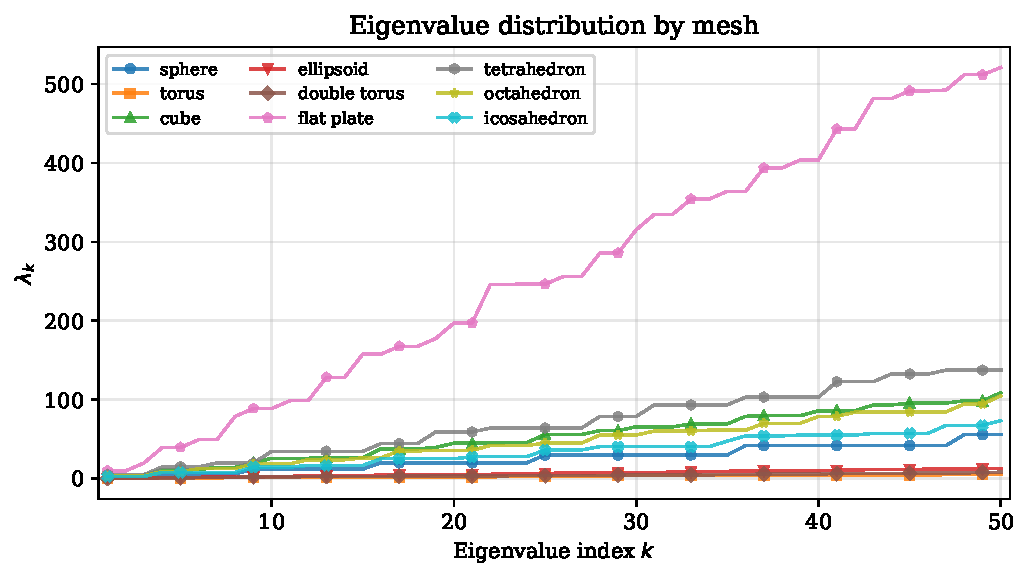
\includegraphics[width=0.85\linewidth]{figures/fig2_eigenvalues.pdf}
\caption{Eigenvalue distributions (first 50 eigenvalues~$\lambda_k$) for the nine meshes. Note the staircase of the sphere (high multiplicity) and the more evenly spaced eigenvalues of the double torus (genus~2). Eigenvalue density and spectral gap vary across shapes, contributing to the distinct visual patterns they produce.}
\label{fig:eigen}
\end{figure}

\subsection{Visual gallery: the same sound, different shapes}
\label{sec:gallery}

Before examining the quantitative structure of the framework, we present visual evidence for the central claim: that the same audio signal, mapped through different eigenbases, yields visually distinct nodal patterns. Figure~\ref{fig:gallery} presents nodal-surface renderings for four shapes (sphere, cube, torus, double torus) and three audio stimuli (A1, A3, A5) using direct mapping. Each panel is annotated with~$\beta_0$ and~$S$.

The pure tone~(A1) produces a clean banded pattern on the sphere (small~$\beta_0$), a face-aligned pattern on the cube and a fragmented mosaic on the double torus. The piano passage~(A3) activates many eigenmodes, producing complex nodal networks on all shapes, most regular on the sphere and most intricate on the double torus. White noise~(A5) produces the most complex pattern in every shape (largest~$\beta_0$), inverting the expectation that an interesting input is needed for an interesting output. Figure~\ref{fig:platonic_gallery} shows nodal patterns on the three Platonic solids for stimuli A1 and A5.

\begin{figure}[!htbp]
\centering
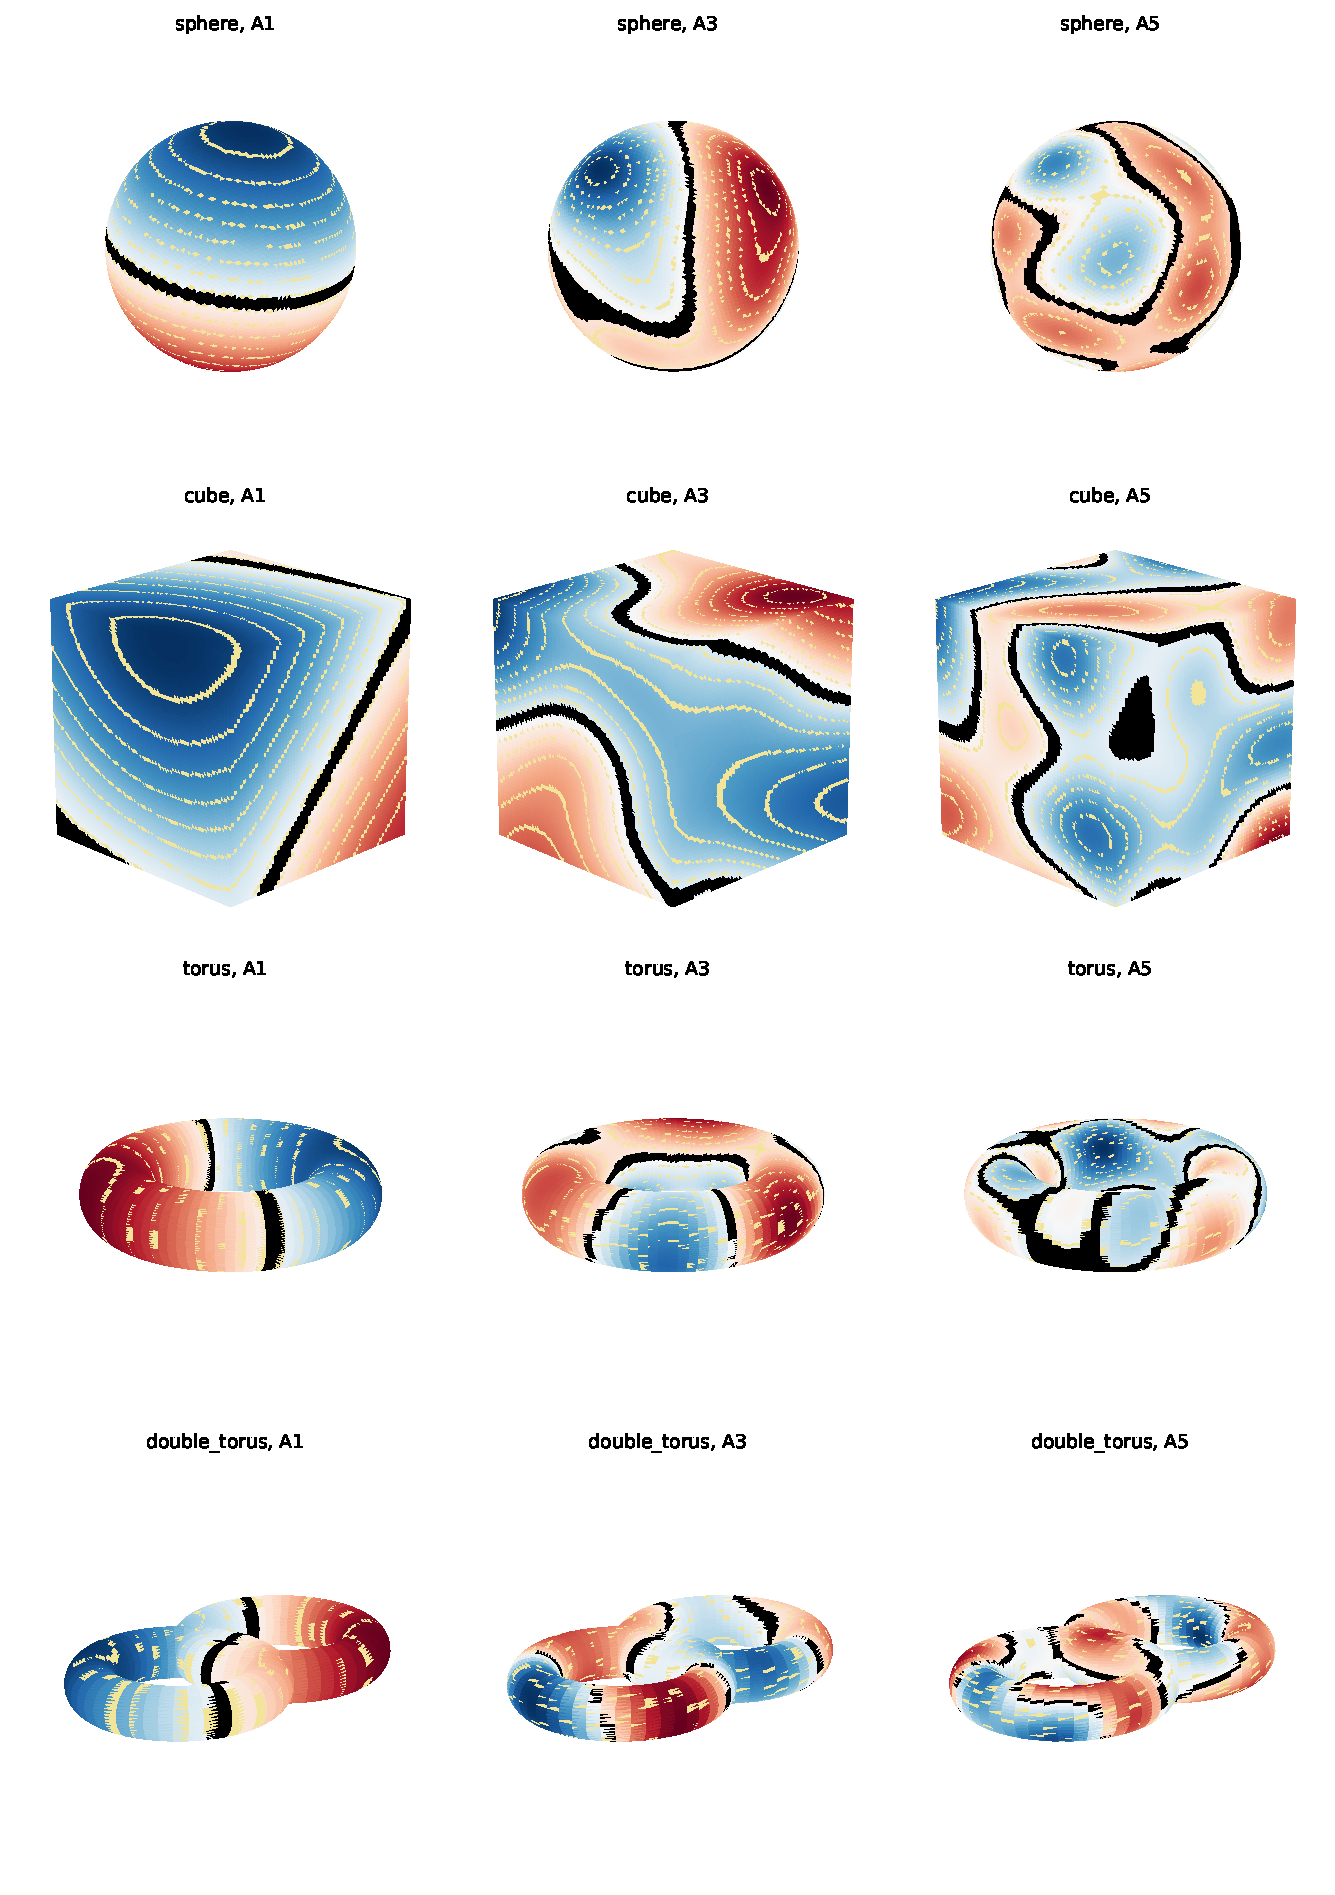
\includegraphics[width=\linewidth]{figures/fig3_nodal_gallery.pdf}
\caption{Nodal-surface gallery: three audio stimuli (A1, A3, A5) mapped onto four shapes (sphere, cube, torus, double torus). Each panel is annotated with~$\beta_0$ and~$S$. The pure tone~(A1) yields a simple banded pattern on the sphere, a face-aligned pattern on the cube, and a fragmented mosaic on the double torus. White noise~(A5) produces the most complex pattern on every shape. These images illustrate the central observation: shape acts as a geometry-dependent spectral filter.}
\label{fig:gallery}
\end{figure}

\begin{figure}[!htbp]
\centering
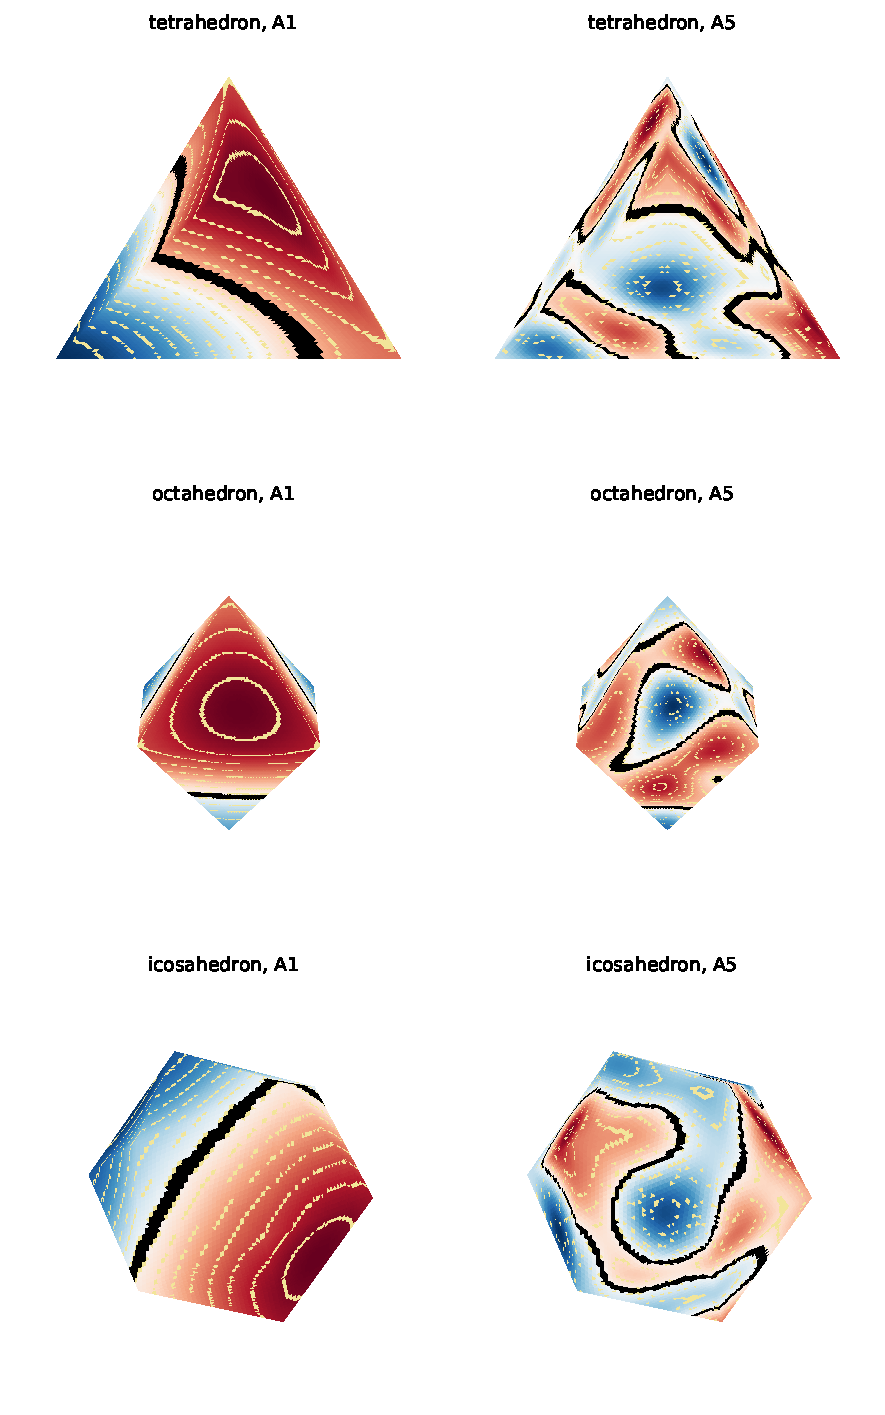
\includegraphics[width=\linewidth]{figures/fig_platonic_gallery.pdf}
\caption{Nodal patterns on the three Platonic solids (tetrahedron, octahedron, icosahedron) for stimuli A1 (pure tone) and A5 (white noise), direct mapping. The discrete symmetry groups impose recognisable geometric motifs---triangular, square, and pentagonal---on the nodal pattern. Each panel is annotated with~$\beta_0$ and~$S$.}
\label{fig:platonic_gallery}
\end{figure}

\subsection{Audio-driven patterns vs.\ random excitation}
\label{sec:random_baseline}

The gallery demonstrates that the patterns are visually striking and shape-dependent, but a prior question remains: does the audio mapping produce nodal patterns that differ \emph{systematically} from those of random excitation? If not, the shape-as-filter metaphor would be vacuous -- every input would produce statistically identical output.

For each of three meshes (sphere, torus, double torus), we draw $N=100$ coefficient vectors uniformly on the unit sphere in~$\mathbb{R}^K$ ($K=50$) and computed $\beta_0$ for each. Figure~\ref{fig:random_vs_audio} compares the resulting baseline (gray band: mean~$\pm\,1\sigma$) with the audio-driven~$\bar{\beta}_0$ for each of the seven stimuli (colored points). The comparison reveals a consistent and interpretable pattern. Spectrally sparse audio (A1, A2) lies well below the random baseline on every mesh (e.g.\ $>5\sigma$ below on the sphere), meaning that a pure tone or triad \emph{simplifies} the nodal pattern relative to random excitation---it activates only a few eigenmodes and thereby produces coherent, legible structure. Broadband audio (A5, white noise) approaches or exceeds the baseline on the torus ($z\approx +2.4$), consistent with white noise that excites all modes roughly equally. The key point is that the audio spectrum selectively activates eigenmodes, shifting~$\beta_0$ in a stimulus-dependent direction; and the \emph{magnitude} of this shift depends on the shape because the eigenbasis determines how the activated modes interfere spatially. This is the operational content of the ``shape as the filter'': the same spectral simplification (sparse audio) produces different amounts of $\beta_0$ reduction on different meshes. The complete deviations per-stimulus, effect sizes, and the distribution of the random-coefficient~$\beta_0$ in three sampling schemes are found in the supplementary material.

\begin{figure}[!htbp]
\centering
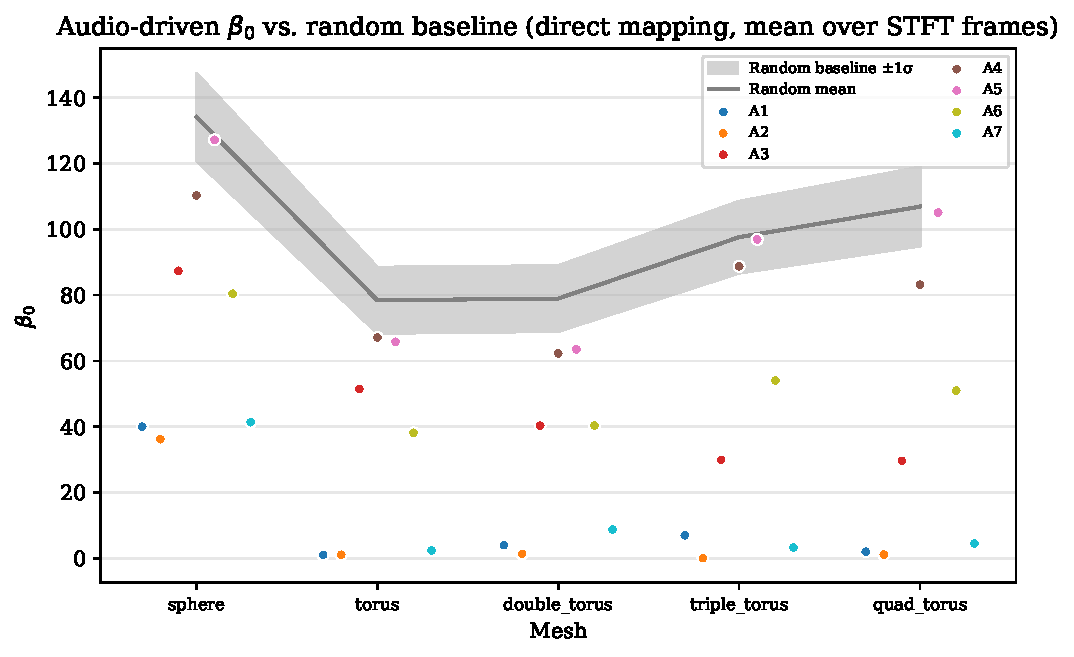
\includegraphics[width=0.85\linewidth]{figures/fig_random_vs_audio.pdf}
\caption{Audio-driven~$\beta_0$ vs.\ random baseline. For each mesh the grey band is the random mean~$\pm\,1\sigma$ ($N=100$, uniform on sphere); coloured points are the seven stimuli (A1--A7, direct mapping, mean over STFT frames). Spectrally sparse audio systematically simplifies the nodal pattern; broadband audio approaches or exceeds the baseline. The magnitude of simplification is shape-dependent.}
\label{fig:random_vs_audio}
\end{figure}

\subsection{Quantitative exploration}
\label{sec:quantitative}

Having established that the patterns are visually differentiated (Section~\ref{sec:gallery}) and statistically distinguishable from random excitation (Section~\ref{sec:random_baseline}), we now examine the quantitative relationships between spectral properties and pattern complexity.

Table~\ref{tab:beta0} reports the time-averaged $\bar{\beta}_0 \pm \sigma(\beta_0)$ on all STFT frames for the direct mapping, for every mesh--audio pair. Static stimuli (A1, A5) show near-zero~$\sigma$; time-varying stimuli (A3, A4, A7) show substantial frame-to-frame variation, confirming that visualization responds to temporal structure. To support the claim that the three mapping strategies (direct, mel-weighted, energy-weighted) are a contribution, Table~\ref{tab:mapping} reports $\bar{\beta}_0$, $A_{\mathrm{ratio}}$, and~$S$ (mean~$\pm$ ~ s.d.\ over all STFT frames) for six representative mesh--audio pairs, with one sub-row per strategy. Figure~\ref{fig:mapping} shows the corresponding nodal patterns for two of these pairs -- torus~$\times$ ~ A3 and double~torus ~ $\times$~A5---with the three strategies side by side, so that the numerical differences can be visually compared. Energy-weighted mapping tends to yield lower~$\beta_0$ and lower~$A_{\mathrm{ratio}}$ than direct or mel-weighted on the same pair (e.g.\ sphere~$\times$~A5, double~torus~$\times$~A5), while mel-weighted can raise~$S$ on time-varying stimuli (e.g.\ torus~$\times$~A3, double~torus~$\times$~A3).

\paragraph{Caveat: temporal autocorrelation}
Consecutive STFT frames overlap (hop~512, window~2048), so $\beta_0$ time series are temporally autocorrelated (lag-1 $r_1 \approx 0.67$ -- $0.92$, $N_{\mathrm{eff}} \approx 38$ -- $169$ vs.\ nominal $N=858$). All summary statistics in Sections~\ref{sec:quantitative}--\ref{sec:temporal} are therefore descriptive, not inferential. Details in the supplementary material.

\begin{table}[t]
\tbl{Mean connected components $\bar{\beta}_0 \pm \sigma$ over all STFT frames (direct mapping). Higher values indicate more fragmented nodal patterns.}
{\begin{tabular}{lccccccc} \toprule
Mesh & A1 & A2 & A3 & A4 & A5 & A6 & A7 \\ \midrule
sphere
  & $52.0\pm0.0$ & $22.5\pm0.8$ & $83.0\pm13.8$ & $112.2\pm25.3$
  & $135.2\pm9.0$ & $60.3\pm8.2$ & $24.4\pm7.3$ \\
torus
  & $0.0\pm0.0$ & $0.0\pm0.0$ & $79.9\pm19.6$ & $105.5\pm28.3$
  & $138.6\pm6.8$ & $46.4\pm7.4$ & $2.9\pm2.8$ \\
cube
  & $49.6\pm0.7$ & $60.9\pm1.0$ & $101.9\pm29.2$ & $196.9\pm56.8$
  & $206.8\pm10.6$ & $82.3\pm20.5$ & $44.9\pm19.1$ \\
ellipsoid
  & $18.0\pm0.0$ & $64.0\pm0.0$ & $82.3\pm17.0$ & $111.6\pm27.2$
  & $140.0\pm7.5$ & $78.3\pm9.8$ & $44.8\pm7.3$ \\
double torus
  & $2.0\pm0.0$ & $2.0\pm0.0$ & $127.4\pm32.9$ & $171.8\pm50.1$
  & $196.6\pm12.9$ & $78.2\pm18.9$ & $4.8\pm2.7$ \\
flat plate
  & $20.0\pm0.0$ & $29.7\pm1.8$ & $54.9\pm9.4$ & $94.7\pm26.5$
  & $129.5\pm9.1$ & $53.0\pm8.3$ & $30.8\pm3.4$ \\
tetrahedron
  & $30.8\pm0.4$ & $18.0\pm0.0$ & $72.5\pm12.4$ & $94.9\pm22.3$
  & $109.9\pm7.6$ & $71.2\pm6.8$ & $28.9\pm8.7$ \\
octahedron
  & $24.0\pm0.0$ & $73.2\pm1.5$ & $100.2\pm15.6$ & $150.1\pm41.6$
  & $162.8\pm8.0$ & $82.5\pm20.6$ & $66.6\pm14.2$ \\
icosahedron
  & $70.0\pm0.0$ & $46.0\pm0.0$ & $78.4\pm14.7$ & $111.8\pm26.5$
  & $129.8\pm7.9$ & $60.2\pm5.4$ & $53.0\pm5.2$ \\
\bottomrule
\end{tabular}}
\label{tab:beta0}
\end{table}

\begin{table}[t]
\tbl{Mapping strategy comparison (representative effects). Energy-weighted mapping tends to yield lower~$\beta_0$ and~$A_{\mathrm{ratio}}$; mel-weighted mapping can raise~$S$ on time-varying stimuli. Full table (six mesh--audio pairs $\times$ three strategies $\times$ three indices) is provided in the supplementary material.}
{\begin{tabular}{llcc} \toprule
Effect & Pair & Direct & Energy-weighted \\ \midrule
$\beta_0$ reduction
  & sphere $\times$ A5 & $135.2 \pm 9.0$ & $91.6 \pm 7.6$ \\
  & double torus $\times$ A5 & $196.6 \pm 12.9$ & $117.5 \pm 13.7$ \\
\addlinespace
  & & Direct & Mel-weighted \\
  \cmidrule(l){3-4}
$S$ increase
  & torus $\times$ A3 & $0.35 \pm 0.03$ & $0.67 \pm 0.13$ \\
  & double torus $\times$ A3 & $0.36 \pm 0.04$ & $0.66 \pm 0.14$ \\
\bottomrule
\end{tabular}}
\label{tab:mapping}
\end{table}

\begin{figure}[!htbp]
\centering
\subfloat[Torus $\times$ A3 (piano). \label{fig:mapping-torus}]{%
  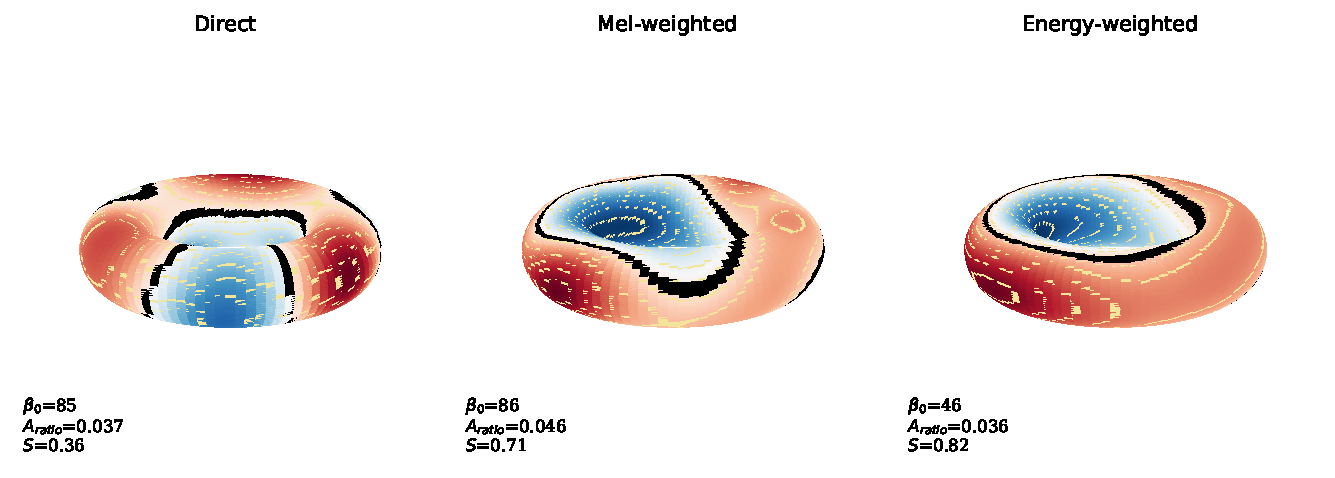
\includegraphics[width=0.8\linewidth]{figures/fig_mapping_comparison.pdf}}\\[1em]
\subfloat[Double torus $\times$ A5 (white noise). \label{fig:mapping-dt}]{%
  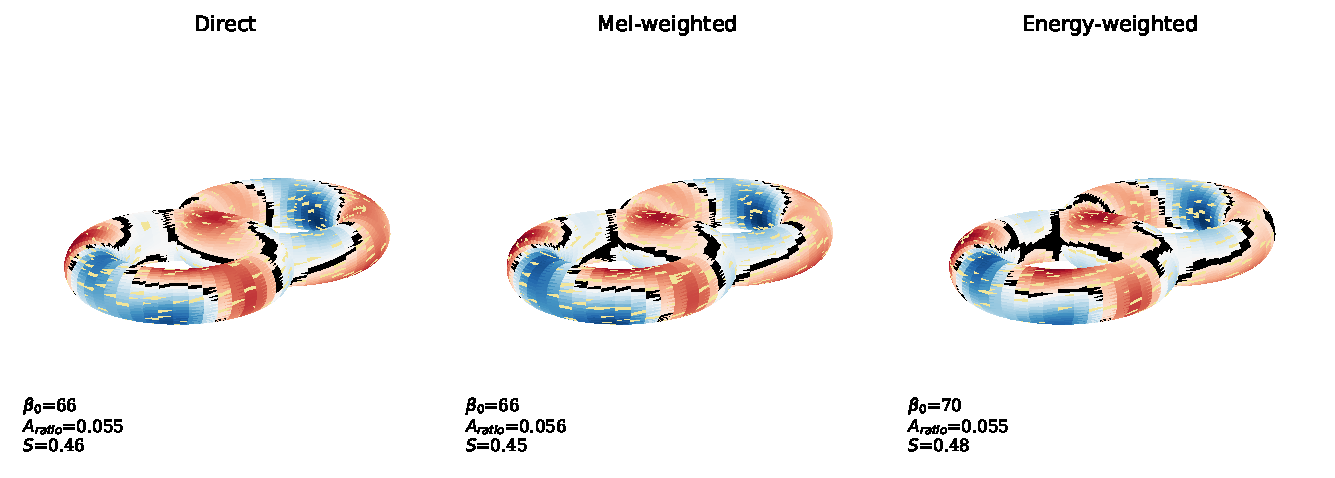
\includegraphics[width=0.8\linewidth]{figures/fig_mapping_comparison_dt.pdf}}
\caption{Visual comparison of the three mapping strategies (direct, mel-weighted, energy-weighted) for two mesh--audio pairs. In each subfigure, the three panels (left to right) show the same scalar field under direct, mel-weighted, and energy-weighted mapping, with shared view and color scale; each panel is annotated with $\beta_0$, $A_{\mathrm{ratio}}$, and~$S$. Energy-weighted (right column) yields smoother, less fragmented patterns (lower $\beta_0$, lower $A_{\mathrm{ratio}}$) than direct or mel-weighted on the same pair, consistent with Table~\ref{tab:mapping}.}
\label{fig:mapping}
\end{figure}

We explore three questions that link spectral properties to pattern complexity.

\paragraph{Spectral gap and pattern onset}
For each mesh, we identify the simplest stimulus (lowest index~$j$) for which $\beta_0>1$ under direct mapping. A large spectral gap~$\gamma$ means that the first mode dominates, so spectrally sparse audio can produce $\beta_0=1$ on shapes with large~$\gamma$ while fragmenting on shapes with small~$\gamma$. A Spearman rank correlation across the nine meshes is consistent with this picture, though $n=9$ is too small for reliable inference.

\paragraph{Symmetry and simple audio}
Comparing~$S$ between high-symmetry meshes (sphere, torus, icosahedron) and lower-symmetry meshes (ellipsoid, flat plate, double torus) for stimuli~A1 and~A2 shows that highly symmetric meshes produce patterns with higher~$S$: the pattern inherits the shape's symmetry when the audio is spectrally simple. For complex audio, the differences in~$S$ diminish.

\paragraph{Eigenvalue density and complexity}
We define a Weyl-like density as the number of eigenvalues per unit range in~$[\lambda_1,\lambda_{50}]$ and examine its correlation with average~$\beta_0$. Meshes with higher density tend to produce higher~$\beta_0$, consistent with the intuition that denser spectra produce more complex interference.

Table~\ref{tab:shapefilter} summarizes how spectral and geometric properties relate to the resulting pattern.

\begin{table}[t]
\tbl{How shape properties influence the nodal pattern (exploratory summary).}
{\begin{tabular}{@{}ll@{}} \toprule
Shape property & Effect on nodal pattern \\ \midrule
Large spectral gap~$\gamma$
  & Simpler patterns for sparse audio; fragmentation onset delayed. \\
High symmetry
  & Pattern inherits symmetry when audio is simple; higher~$S$. \\
High eigenvalue density
  & More complex patterns; higher~$\beta_0$ on average. \\
Low symmetry / high genus
  & More fragmented, asymmetric patterns; lower~$S$. \\
\bottomrule
\end{tabular}}
\label{tab:shapefilter}
\end{table}

\subsection{Genus and topological complexity}
\label{sec:genus}

Section~\ref{sec:quantitative} showed that the density of the eigenvalues correlates with the complexity of the pattern in our nine meshes. However, eigenvalue density is itself shaped by multiple geometric factors---curvature distribution, symmetry, and topology---so it need not be determined by any single one. A natural follow-up is whether the \emph{topology} of the shape, specifically its genus, drives this density, and hence predicts the complexity of the nodal pattern. If higher-genus shapes systematically offer denser and less degenerate spectra, one might expect monotonically increasing fragmentation with genus.

We constructed a seven-point genus sequence at comparable resolution (${\sim}5{,}000$ vertices): sphere (genus~0), torus (genus~1), double torus (genus~2) and surfaces of genus~3 through~6. The plot of~$\beta_0$ against genus under direct mapping is provided in the supplementary material. The result is \emph{not} monotonic. The sphere (genus~0) yields $\beta_0=26$; the torus (genus~1) attains $\beta_0=0$ for spectrally simple stimuli (A1, A2); the double torus (genus~2) yields $\beta_0=1$; and the genus~3--6 surfaces yield $\beta_0 = 42$, 58, 40 and 38 respectively (complete data in the supplementary material).

The torus anomaly admits a concrete explanation. On a \emph{flat} torus $\mathbb{R}^2/\Gamma$ the eigenvalues are $\lambda = (m/R)^2 + (n/r)^2$; our mesh is an embedded torus in $\mathbb{R}^3$ with non-zero curvature, so that formula does not apply exactly, but mode analysis confirms that for A1 and A2 the dominant modes correspond to the $(m,n)=(1,0)$ doublet in that flat torus picture. Any linear combination of this doublet has a single nodal curve winding once around the torus -- a direct consequence of the product geometry separating longitudinal and meridional modes.

This non-monotonic result shows that the genus alone does not control~$\beta_0$; the \emph{distribution} of eigenvalues matters. While the preceding subsections examined three separate spectral predictors (spectral gap, symmetry, eigenvalue density), each capturing one aspect of the spectrum, we need a single descriptor that integrates eigenvalue spacing into a unified measure. This is the subject of the next section.


%% ====================================================================
\section{Spectral entropy: from topology to a unifying descriptor}
\label{sec:spectral_entropy}
%% ====================================================================

The non-monotonic genus--$\beta_0$ relationship of the preceding section raises a theoretical question that extends beyond the immediate goals of the generative framework. Although Section~\ref{sec:quantitative} treated the spectral gap, symmetry, and eigenvalue density as separate predictors, we now ask whether a single spectral quantity can account for the data -- including anomalies that genus alone cannot explain. This section introduces such a quantity and formulates an open question for the spectral-geometry community.

\subsection{Definition and motivation}
\label{sec:entropy_def}

For a random linear combination of eigenfunctions in a \emph{single} eigenspace of degree~$L$ on the sphere, \citet{nazarov2009} proved that the expected number of \emph{nodal domains} (connected components of the complement of the nodal set) grows as $\mathbb{E}[\mathcal{N}] \sim c\,L^2$. Our index~$\beta_0$ counts connected components of the nodal set itself (Section~\ref{sec:indices}), not the nodal domains; in~$S^2$ both scale as~$L^2$, but the quantities and constants differ. However, our audio-driven fields are \emph{finite superpositions across multiple eigenspaces---a} fundamentally different setting for which no analog is known. This gap in the literature on the nodal-domain motivates the following descriptor.

We define the \emph{spectral entropy} of the activated eigenvalue range $[\lambda_1,\lambda_K]$ as
\[
  H \;=\; -\sum_{k=1}^{K-1} p_k \ln p_k, \qquad
  p_k = \frac{\lambda_{k+1}-\lambda_k}{\lambda_K - \lambda_1},
\]
which measures the uniformity of the eigenvalue spacing. High spectral entropy corresponds to evenly spaced, non-degenerate eigenvalues (as on the double torus), producing complex interference and high fragmentation; low entropy corresponds to clustered, highly degenerate eigenvalues (as on the sphere or the torus with its product geometry), producing coherent nodal patterns and lower~$\beta_0$---even when the genus is higher.

\subsection{Empirical evidence and an open question}
\label{sec:entropy_evidence}

The plot of $H$ against mean~$\beta_0$ (random coefficients, $N=200$ samples per mesh) for all 13 meshes in $K=50$ is provided in the supplementary material. The Spearman rank correlation is $\rho \approx +0.71$ ($n=7$, genus sequence, $p\approx0.07$) and $\rho \approx +0.4$ ($n=9$, direct mapping of A5). With $n=7$ the former does not reach conventional significance; therefore, we regard the relationship as empirically motivated rather than confirmed.

These data suggest a question that we offer as a target for analytic investigation rather than as a formal conjecture, given the limited sample size:

\paragraph{Open question}
\label{conj:spectral_entropy}
For a linear combination $f = \sum_{k=1}^{K} a_k\,\phi_k$ on a closed orientable surface of genus~$g$, with coefficients drawn uniformly from the unit sphere in~$\mathbb{R}^K$, does the expected number of connected components~$\mathbb{E}[\beta_0]$ increase monotonically with~$H$ for fixed~$K$? More generally, for \emph{a random linear combination $f=\sum_{k=1}^K a_k\phi_k$ on a closed surface, how does $\mathbb{E}[\beta_0]$ depend on the sequence of eigenvalues $\{\lambda_k\}$ and the genus?}

A sensitivity sweep over $K\in\{50,100,200\}$ and three coefficient sources (random, A5, A3) confirms that the rank ordering is qualitatively stable; the non-monotonic genus--$\beta_0$ relationship and the torus anomaly persist at all tested~$K$ (supplementary material). The complete spectral-descriptor analysis (effective multiplicity, product-structure score, $\varepsilon$-robustness), stem plots of eigenvalues, mesh-quality metrics, the Nazarov--Sodin comparison on the sphere and random-distribution coefficient~$\beta_0$ baselines are provided in the supplementary material.

Regardless of whether this question admits a clean analytic answer, spectral entropy serves a practical role in the generative framework: it provides a single number that predicts, better than genus or any of the individual spectral descriptors of Section~\ref{sec:quantitative}, how visually complex a given shape will render a typical audio input. An artist choosing among shapes can consult~$H$ as a guide to the expected visual register, a point we return to in Section~\ref{sec:artistic}.


%% ====================================================================
\section{Temporal dynamics and compositional use}
\label{sec:temporal_compositional}
%% ====================================================================

The analyzes so far have treated each shape--audio pair as a static summary: a single $\bar{\beta}_0$ averaged over all STFT frames. But music is a temporal art and a framework for audio visualization must demonstrate that it responds to the temporal structure of sound. This section examines the full temporal trajectory of~$\beta_0$ (Section~\ref{sec:temporal}), and then shows how the time-varying responsiveness documented there enables a compositional practice in which shapes are \emph{sequenced} against audio to produce visual narratives (Section~\ref{sec:sequencing}).

\subsection{Temporal persistence of nodal topology: capturing audio dynamics}
\label{sec:temporal}

We analyze time-varying stimuli (A3, A4, A7) with overlapping STFT frames (hop~512), computing $\beta_0$ per frame on the sphere and the torus. Figure~\ref{fig:temporal} plots the resulting time series. To relate $\beta_0$ variation to concrete audio events, we align the time series with the RMS envelope per-frame and the spectral flux (frame-to-frame change in the magnitude spectrum) on the same STFT grid. The alignment for the piano (A3) stimulus (RMS envelope, spectral flux, and $\beta_0$ for sphere and torus on a shared time axis) is provided in the supplementary material. In the sphere, $\beta_0$ correlates with RMS (A3: Spearman $\rho=0.19$, $p<0.001$; A7: Pearson $r=0.29$, $p<0.001$), so louder or denser passages tend to coincide with greater fragmentation; the analogous plot for A7 is provided in the supplementary material.

To identify which audio features drive these fluctuations, we computed correlations between the $\beta_0$ time series and four per-frame audio descriptors (RMS energy, spectral flux, spectral centroid, number of active frequency bins) for A3 and A7 in the sphere and torus. The strongest correlate varies by condition: on the sphere, the number of active bins best predicts $\beta_0$ (Spearman $\rho$ up to $0.84$); on the torus, the RMS energy is a stronger predictor for A3 ($\rho=0.65$). Cross-correlation analysis reveals that $\beta_0$ can delay the audio by several frames in some conditions. The full correlation tables (Pearson, Spearman, cross-correlation at lags $-5$ to $+5$) are provided in the supplementary material. The overlay plots of $\beta_0$ with the best-correlated descriptor and cross-correlation versus lag are provided in the supplementary material.

\begin{figure}[!htbp]
\centering
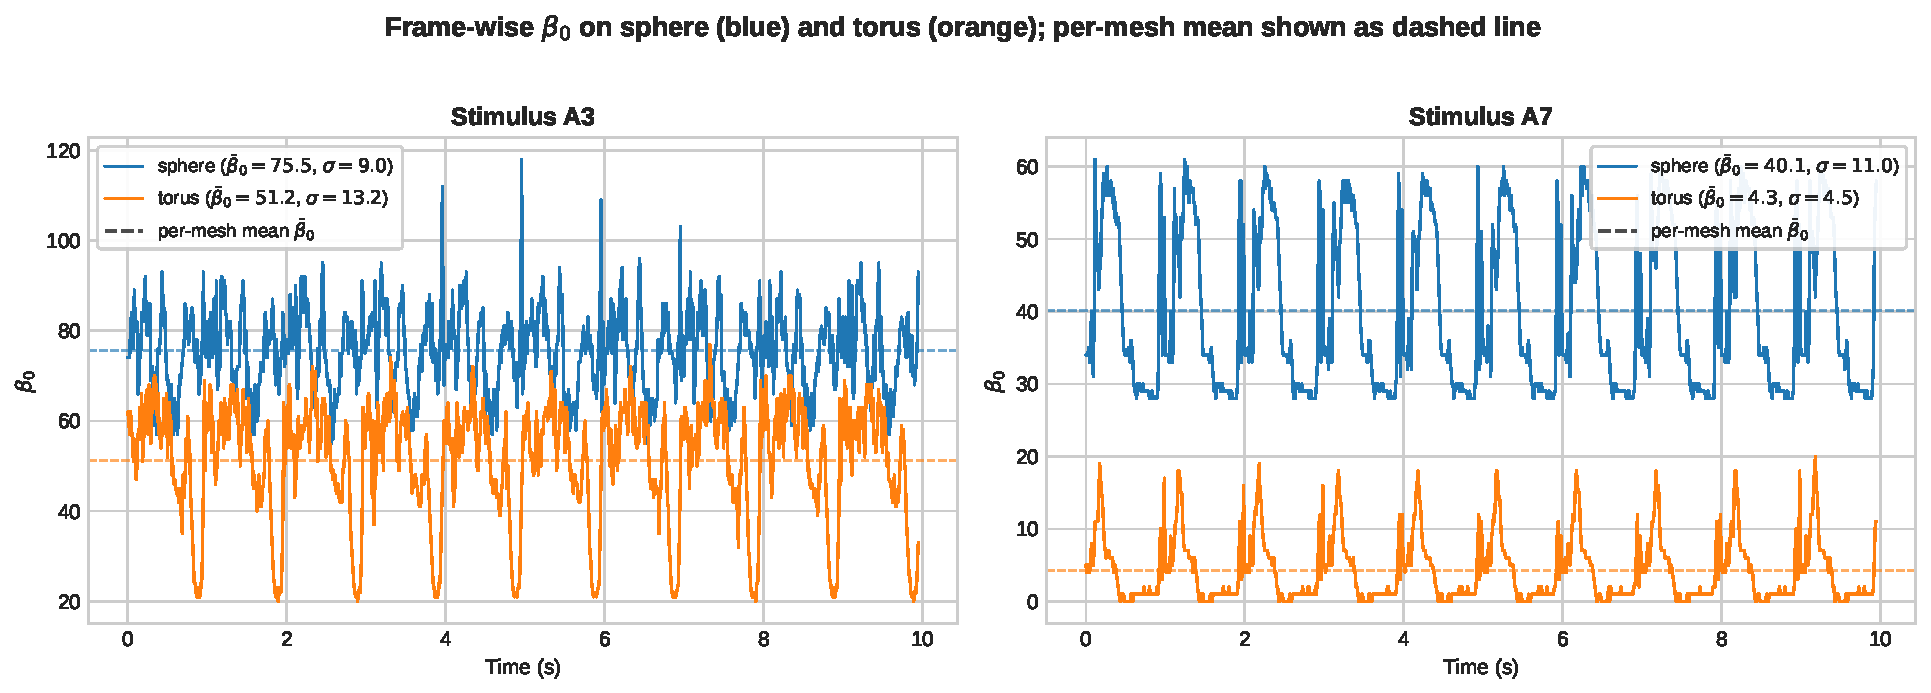
\includegraphics[width=0.75\linewidth]{figures/fig_temporal_persistence.pdf}
\caption{Frame-by-frame~$\beta_0$ over the piano passage~(A3) on the sphere (blue) and the torus (orange). The sphere shows moderate fluctuation ($\sigma\approx9.0$), tracking the temporal dynamics of the piano; the torus shows $\bar{\beta}_0\approx51$ with $\sigma\approx13.2$.}
\label{fig:temporal}
\end{figure}

\begin{figure}[!htbp]
\centering
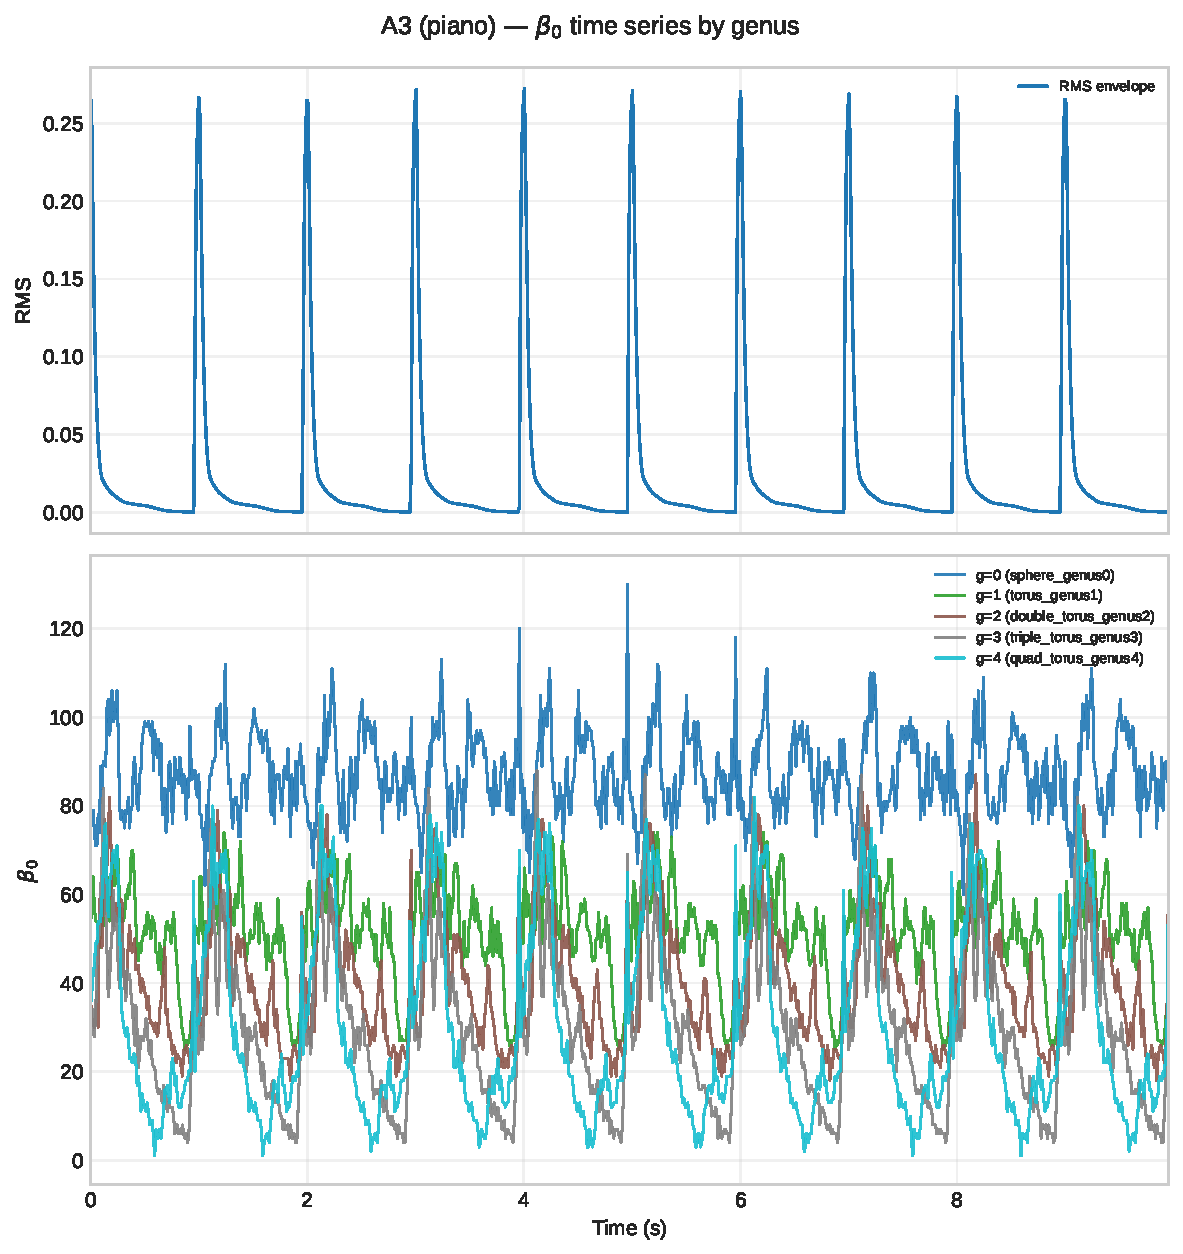
\includegraphics[width=0.85\linewidth]{figures/fig_temporal_genus.pdf}
\caption{Frame-by-frame $\beta_0$ for A3 (piano) on the genus sequence (sphere, torus, double torus; genus~3 and~4 when available), with RMS envelope (top). Same STFT grid and time axis; higher-genus meshes show greater temporal variance.}
\label{fig:temporal_genus}
\end{figure}

\begin{figure}[!htbp]
\centering
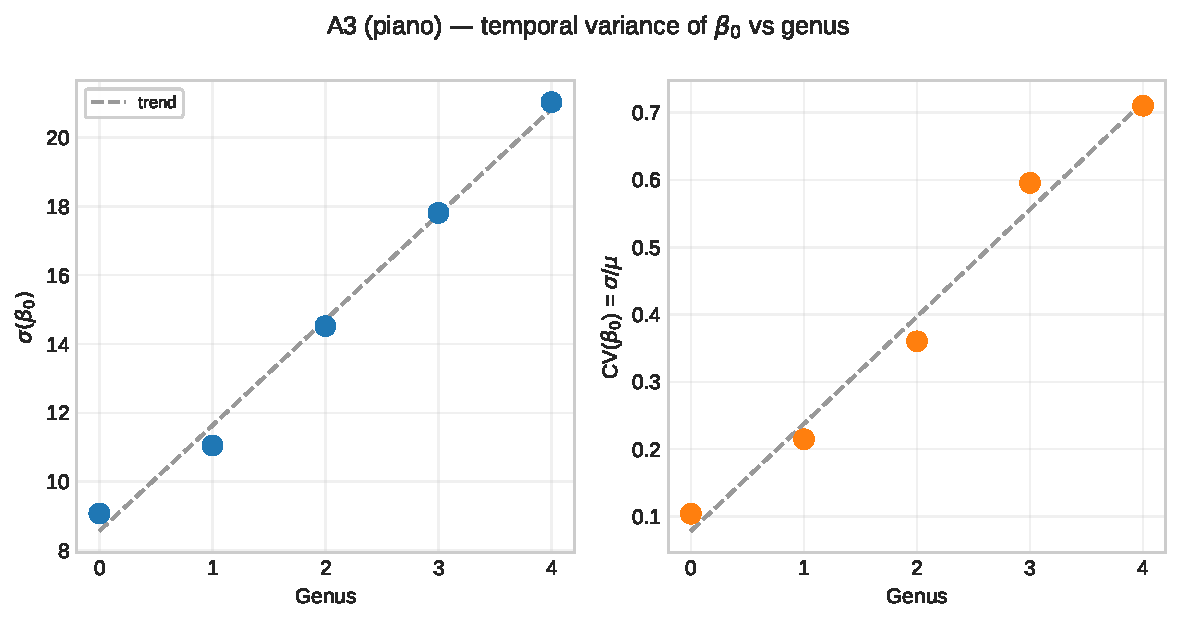
\includegraphics[width=0.85\linewidth]{figures/fig_temporal_variance_vs_genus.pdf}
\caption{Temporal variance of $\beta_0$ vs.\ genus for A3 (piano): $\sigma(\beta_0)$ (left) and CV($\beta_0$) (right). In the genus sequence, both increase with genus in the run shown (0--2), indicating that higher-genus shapes exhibit stronger frame-to-frame fluctuation of the nodal topology.}
\label{fig:temporal_variance_genus}
\end{figure}

In the genus-sequence meshes (${\sim}5{,}000$ vertices, 858 frames), A3 yields $\bar{\beta}_0 = 75.5\;(\sigma=9.0)$ on the sphere and $51.2\;(\sigma=13.2)$ on the torus; the absolute values are lower than in Table~\ref{tab:beta0} due to the coarser resolution (${\sim}5{,}000$ vs.\ ${\sim}10{,}000$ vertices; the convergence test in Section~\ref{sec:method} indicates that halving the vertex count reduces~$\beta_0$ by roughly 20--30\% in absolute terms while preserving rank ordering across meshes). Extending to the full sequence of genus (Figures~\ref{fig:temporal_genus} and~\ref{fig:temporal_variance_genus}), the temporal variance of $\beta_0$ increases with the genus---$\sigma$ increases from $9.0$ (sphere) to $15.3$ (double torus) and CV from $0.12$ to $0.30$---indicating that shapes of higher-genus exhibit greater frame-to-frame fluctuation of the nodal topology.

\paragraph{Sensitivity to~$K$}
A sensitivity analysis for $K\in\{10,50,100,200\}$ confirms that the non-monotonic genus--$\beta_0$ relationship and the torus anomaly persist in all tested~$K$ (supplementary material).

\subsection{Shape sequencing: composing with geometry}
\label{sec:sequencing}

The temporal analysis above established that the nodal pattern tracks the audio dynamics in a shape-dependent manner: different shapes amplify different temporal features and exhibit different degrees of frame-to-frame variability. This responsiveness is precisely what makes shape sequencing viable as a compositional tool -- if the pattern were static, switching shapes mid-stream would produce an abrupt visual substitution rather than an organic transition.

We composed a short visual study using the piano stimulus~(A3) and three shapes in succession: sphere during the sparse opening, torus as the harmonic density increases, and double torus for the climax. Figure~\ref{fig:shape_sequencing} documents this composition: three representative STFT frames: a sparse frame near the opening (frame~50, low RMS), the frame of maximum RMS (frame~345), and a quiet frame after the climax (frame~426) -- delivered in all three shapes. The visual arc is immediate: the sphere's smooth bands give way to the torus's woven lattice, which in turn dissolves into the double torus's fragmented mosaic. The transition from torus to double torus at the climax is the most striking moment---the grid structure that had provided visual coherence suddenly breaks apart, and the resulting visual rupture parallels the harmonic saturation of the piano's fortissimo. These transitions function as visual analogs of orchestral changes: just as a composer moves from strings to full orchestra to control textural density, the practitioner moves from sphere to double torus to control visual complexity.

\begin{figure}[!htbp]
\centering
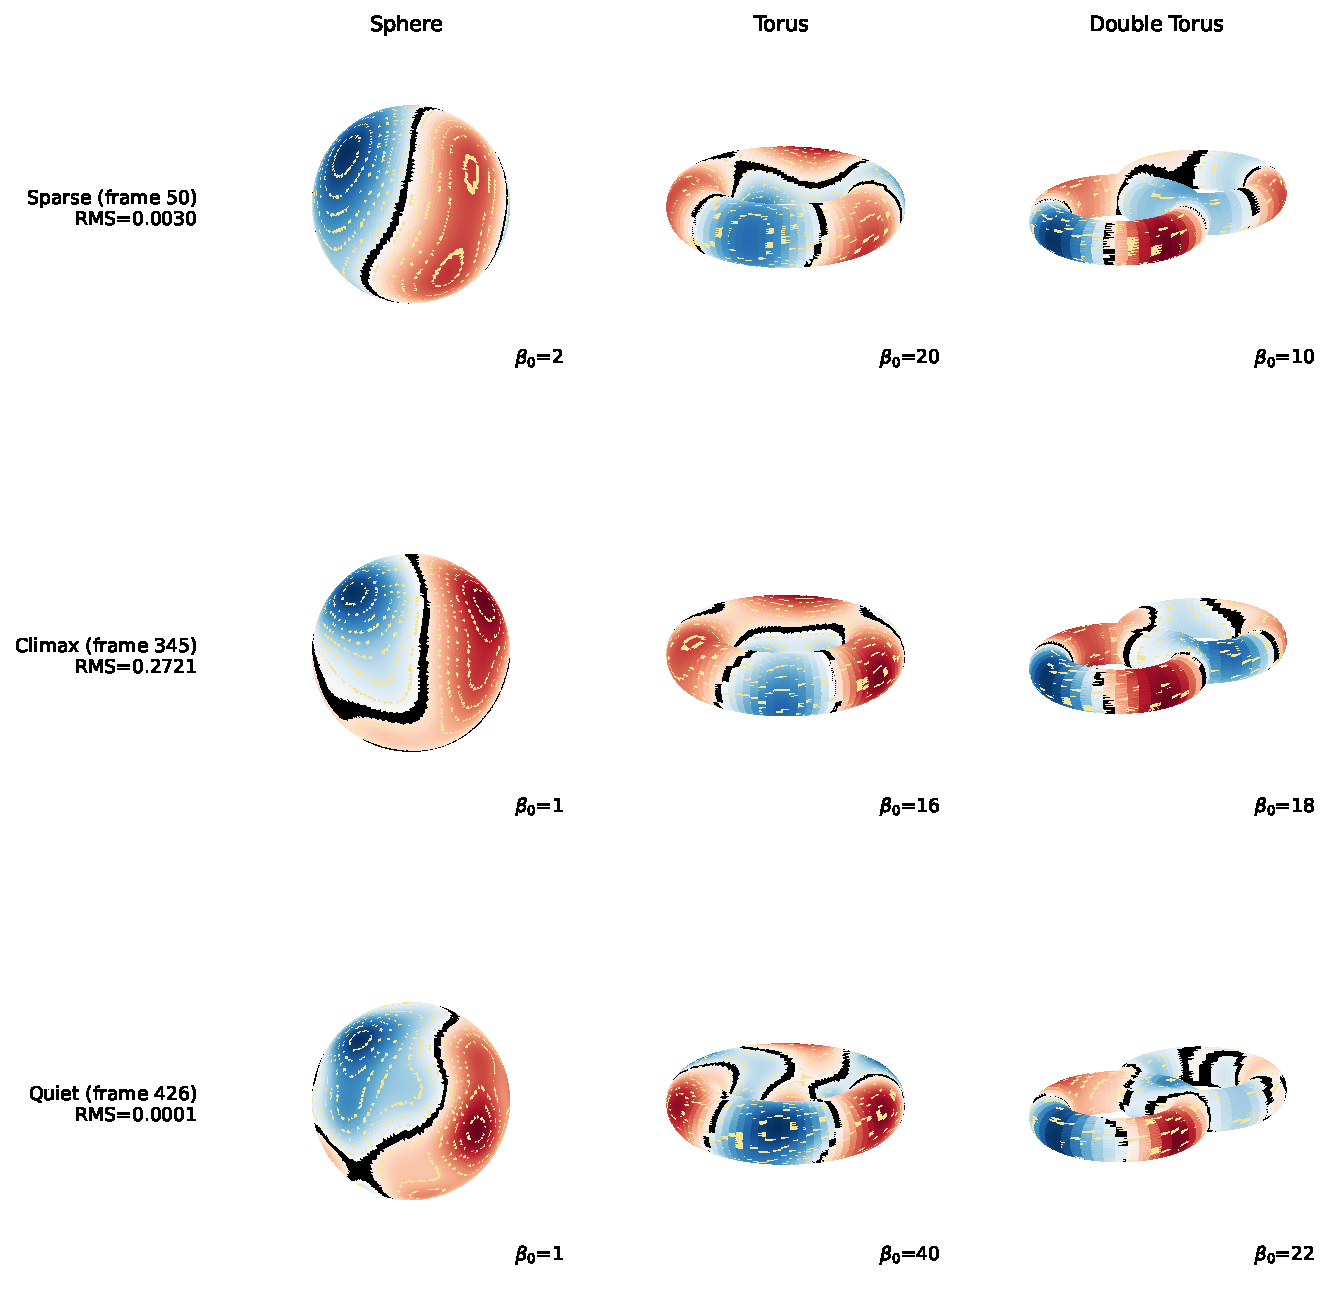
\includegraphics[width=0.95\linewidth]{figures/fig_shape_sequencing.pdf}
\caption{Shape sequencing: the same piano passage~(A3) on three shapes for three representative frames. Rows: sparse (frame~50, low RMS), climax (frame~345, maximum RMS), quiet (frame~426, local RMS minimum after climax). Columns: sphere, torus, double torus. Each panel shows the scalar field (diverging colormap) with the nodal set ($|f|<\varepsilon$) in black; $\beta_0$ is annotated. The same audio yields visually distinct nodal patterns on each shape, and $\beta_0$ varies by both frame type and shape (e.g.\ torus $\beta_0=20$ at sparse, 16 at climax, 40 at quiet).}
\label{fig:shape_sequencing}
\end{figure}

The same approach applied to the cello excerpt~(A7) (four phrase-boundary frames on the same three shapes) is documented in the supplementary material. The cello's narrower spectral bandwidth produces subtler shape-dependent differences than the piano---the sphere and torus remain relatively sparse throughout---but the double torus registers the timbral shift between lyrical and forceful bowing as a visible change in nodal density, demonstrating that the framework can capture not only harmonic complexity but also timbral nuance.

These two sequencing studies serve as proof of concept for a compositional practice whose artistic implications we discuss in Section~\ref{sec:artistic}.


%% ====================================================================
\section{Shape selection as a generative parameter}
\label{sec:artistic}
%% ====================================================================

The preceding sections have documented the framework's behavior empirically, how spectral properties predict pattern complexity (Section~\ref{sec:exploration}), how spectral entropy unifies these predictors (Section~\ref{sec:spectral_entropy}), and how temporal dynamics enable compositional use (Section~\ref{sec:temporal_compositional}). We now shift perspective from \emph{what the framework produces} to \emph{what it offers as a generative methodology}. This section is primarily addressed to the practitioner; the mathematical reader may find the open question of Section~\ref{sec:spectral_entropy} more engaging.

The key distinction from extrinsic audio-visualization systems (Section~\ref{sec:related}) is that here the mapping is \emph{intrinsic}: switching from a sphere to a double torus changes the eigenbasis and hence every aspect of the visual output. The artist's decision is not ``which audio feature drives which visual parameter?''\ but ``which geometric filter do I want to apply to the entire audio spectrum?''

\subsection{Shape selection in the context of generative systems}

In generative systems, the designer's role often lies not in specifying the output directly but in choosing the rules that produce it. The choice of tiling rule determines the output of a substitution system \citep{trevio2022}; the choice of symmetry group determines the structure of a wallpaper pattern \citep{goldstine2017}; the choice of tuning system shapes the color of musical intervals \citep{sethares1998}. In our framework, the analogous decision is the choice of mesh. Selecting a sphere means choosing high symmetry and degenerate eigenvalues; selecting a double torus means choosing richer topology and denser spectra. The user need not know the Laplace--Beltrami operator to make this choice meaningfully---the visual difference is immediately apparent in the interactive application---but the mathematical framework explains \emph{why} the difference exists and allows one to anticipate, at least qualitatively, what kind of visual transformation each shape will impose.

This positions shape selection alongside other mathematically grounded generative parameters. Just as an understanding of equal temperament versus just intonation enriches a composer's harmonic palette, an understanding of spectral gap versus eigenvalue density---tentatively summarized by spectral entropy~$H$ (Section~\ref{sec:spectral_entropy}), pending validation on a larger mesh collection---enriches the visual palette available in this framework. The shape-sequencing studies of Section~\ref{sec:sequencing} demonstrate this concretely: sequencing shapes against a fixed audio track produces a visual narrative in which shape transitions function as expressive decisions with mathematically grounded consequences, and the web application (Section~\ref{sec:interactive}) supports real-time shape switching to make this practice immediately accessible.

\subsection{Visual character across the shape palette}
\label{sec:visual_character}

The gallery (Section~\ref{sec:gallery}) and quantitative analysis (Section~\ref{sec:quantitative}) established the factual basis: different shapes produce different patterns with measurably different~$\beta_0$, $A_{\mathrm{ratio}}$ and~$S$. Here, we interpret these differences as a \emph{visual vocabulary}, a palette of registers that a practitioner can draw upon.

The \textbf{sphere} acts as a \emph{smoothing filter}. Its degenerate eigenvalues merge many modes into coherent bands, producing patterns with long, flowing nodal curves that wrap the surface like contour lines on a globe. Even complex audio yields a sense of global order---a visual calm that persists regardless of acoustic turbulence. This register of continuity and legibility suits audio that the viewer should be able to ``read'': a melodic line, a slow harmonic progression.

The \textbf{torus} acts as a \emph{lattice filter}. Its product geometry favors grid-like nodal networks whose longitudinal and meridional components echo the two independent cycles of the surface. For spectrally simple audio, the nodal set collapses to a single connected curve ($\beta_0=0$) -- a moment of striking visual economy. Complex audio breaks the network into an interlocking weave, but the underlying grid structure remains perceptible as a visual rhythm. This register of periodicity and woven texture suits audio with repetitive or layered structure: ostinato patterns, polyrhythmic textures.

The \textbf{double torus} and higher-genus surfaces act as \emph{fragmentation filters}. Their denser and less degenerate spectra (higher~$H$) distribute energy across many independent modes, producing mosaic-like patterns with high~$\beta_0$. The visual effect is one of fine-grained texture: the nodal curves form a dense, irregular network that fills the surface without a dominant direction or scale. This register of density and local complexity suits harmonically rich audio--orchestral tutti, noise textures--where the visual density matches the acoustic density.

The \textbf{Platonic solids} occupy an intermediate position. Their discrete symmetry groups impose recognizable geometric motifs on the nodal pattern, producing a quality of stained glass or tiled pavement where the regularity of the underlying geometry frames the irregularity of the audio-driven field. The choice among them--the tetrahedron for stark, angular patterns; icosahedron for rounder, more intricate ones--is a choice of visual temperament as much as of mathematical structure.

These characterizations are tendencies modulated by the mapping strategy and the audio's spectral content, but they suggest that one can develop a working intuition for ``what this shape will do to my sound.'' More generally, shape selection functions as a \emph{visual register} whose affordances are predicted by the spectral analysis and summarized by~$H$; the artistic decision---which register to use when and how to sequence transitions---remains with the practitioner.

\subsection{Observations from the design process}
\label{sec:observations}

The quantitative results above describe the framework's behavior; this subsection records how those results emerged through iterative exploration---a reflection on the design process itself, in the spirit of the practice-based accounts given by \citet{feijs2019} and \citet{dorfsmanhopkins2021}.

\paragraph{Shape dominates audio as a source of visual character.}
The most consequential discovery was that shape selection proved to be a stronger determinant of visual character than audio content---a sine tone on the double torus was visually richer than a Bach fugue on the sphere. This finding, which emerged only through real-time experimentation with the interactive tool, reoriented the project toward the ``shape as the spectral filter'' framing. In the sense of \citet{dorfsmanhopkins2021}, the visual output raised a question (why does shape dominate?) that the mathematics then answered (because the eigenbasis, not the coefficient vector, controls the spatial structure of interference).

\paragraph{Temporal ``breathing'' in real time.}
Transitioning between shapes while the same audio plays produces a visually compelling experience in which the viewer perceives the shape as an active agent transforming the sound. The temporal ``breathing'' documented in Section~\ref{sec:temporal} is perceptually striking in real time: the nodal pattern feels \emph{responsive} to the music rather than merely correlated with it.

\paragraph{Mapping strategies as a secondary parameter.}
The three strategies were not designed simultaneously. The direct mapping came first as the simplest choice, but early visual tests revealed that it often under-represented perceptually important mid-range frequencies. The mel-weighted mapping was introduced to address this, and the energy-weighted mapping followed when we sought stronger visual contrasts for live demonstration. In practice, direct mapping preserves frequency ordering and produces patterns with a clear low-to-high spatial gradient; mel-weighted mapping compresses high frequencies and emphasizes perceptually salient structure; energy-weighted mapping amplifies contrasts and produces bolder nodal boundaries.

\paragraph{Informative failures.}
Not all shape--audio combinations produced compelling results. The ellipsoid under white noise~(A5) yielded a densely fragmented pattern visually indistinguishable from random stippling---complex in the $\beta_0$ sense but monotonous to the eye, lacking the spatial organization that makes the sphere's bands or the torus's lattice legible. The flat plate with simple audio (A1, A2) closely resembled textbook two-dimensional Chladni figures, offering little beyond the classical setup. These failures sharpened our sense of when three-dimensional geometry adds genuine visual value: it is most effective when the shape has enough curvature variation or topological complexity to impose a recognizable spatial vocabulary, but not so much spectral density that the pattern collapses into undifferentiated noise. The ``sweet spot''---the torus, the Platonic solids, the double torus under moderately rich audio---emerged from repeated visual comparison in the interactive tool, a process closer to the iterative aesthetic judgment described by \citet{feijs2019} than to hypothesis testing.

\paragraph{Rendering as a further parameter.}
A further generative parameter, still fixed in the quantitative analysis, is the \emph{rendering configuration}: color map, lighting, camera angle, and threshold~$\varepsilon$. After testing several schemes---sequential (viridis), warm diverging (brown--cream--teal), and high-contrast (black--gold--black)---we adopted a divergent blue--white--red colormap because it renders the sign change as a legible color boundary across all nine meshes, making the nodal set's topological structure immediately visible. This choice prioritized robustness across shapes over personal preference for any single mesh.

%% ====================================================================
\section{Interactive web application}
\label{sec:interactive}
%% ====================================================================

An interactive web application (Figure~\ref{fig:demo}), built with Vite, React, and Three.js, loads a mesh and its precomputed eigenbasis, captures audio from the microphone or an audio file, performs the STFT--mapping--field computation in real time, and renders the scalar field as a color map with the nodal set highlighted. The interface presents a 3D viewport (WebGL, Three.js) flanked by a control panel. The user selects a mesh from a dropdown menu (nine meshes, loadable in less than 0.5 \, s), chooses a mapping strategy (direct, mel, energy) and enables microphone input or loads an audio file. The scalar field is recomputed for each STFT frame (${\approx}86$\,Hz) and rendered as a vertex-colored mesh with the approximate nodal set highlighted in black; latency from audio input to visual update is less than 20 \, ms on a mid-range laptop (tested: Apple~M1, Chrome~120). The three indices ($\beta_0$, $A_{\mathrm{ratio}}$, $S$) are displayed numerically and updated in real time. Crucially, switching shapes while the same audio plays, a single click, offers an immediate demonstration of the geometry-dependent filter: the pattern reorganizes within one frame, making the mathematical content of Section~\ref{sec:background} tangible without requiring the user to engage with the formalism directly. The application logs interaction events (mesh switches, audio changes, timestamps) to support future controlled user studies.

The application is available at \url{https://joonhyungbae.github.io/Sonifold/} and the source code at \url{https://github.com/joonhyungbae/Sonifold}. Beyond individual exploration, we envision three deployment contexts: (i)~a \emph{live performance} setting in which a performer sequences shapes against a live audio feed, using shape transitions as expressive gestures analogous to changes in orchestration; (ii)~an \emph{installation} in which a fixed mesh responds to ambient sound, so that the nodal pattern registers the acoustic environment of the gallery in real time; and (iii)~a \emph{pedagogical} tool for spectral geometry courses, where students can see how eigenvalue multiplicity, spectral gap, and genus affect nodal patterns without writing code.

\begin{figure}[!htbp]
\centering
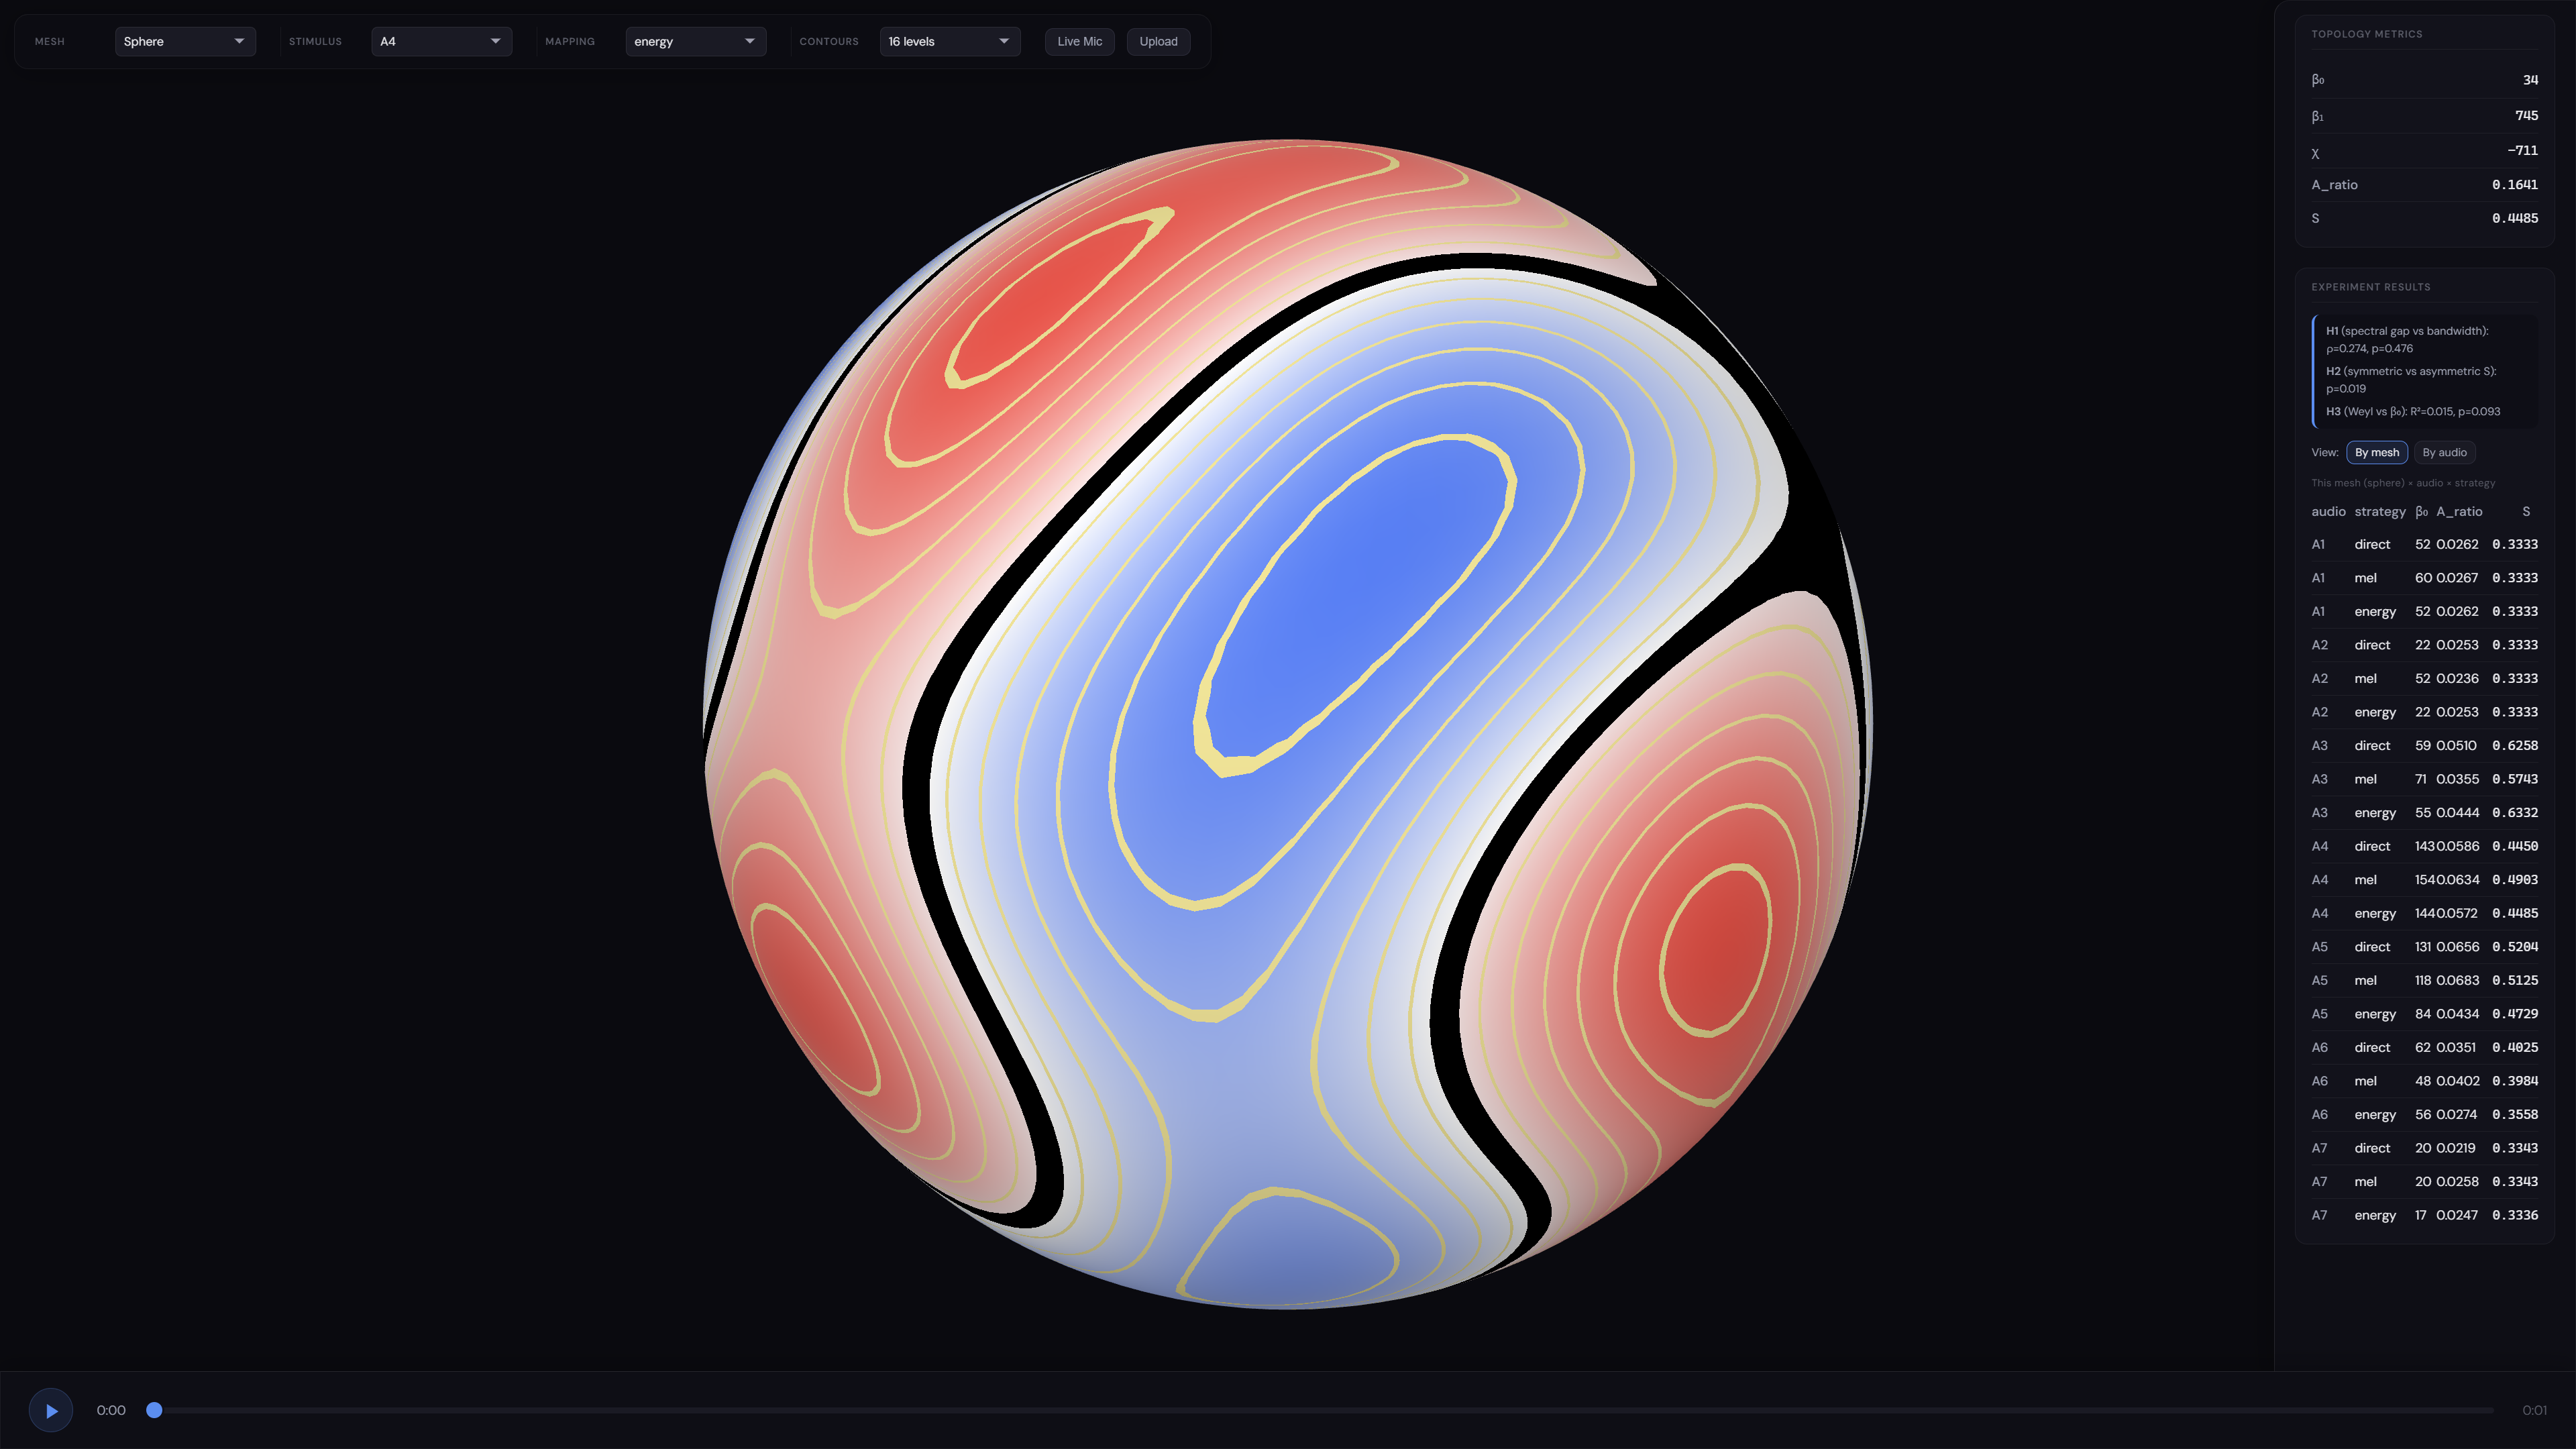
\includegraphics[width=0.75\linewidth]{figures/web.png}
\caption{Screenshot of the interactive web application. The user selects a mesh and mapping strategy; live audio drives the scalar field in real time. Switching shapes while the same audio plays offers an immediate demonstration of the geometry-dependent filter.}
\label{fig:demo}
\end{figure}

%% ====================================================================
\section{Discussion}
\label{sec:discussion}
%% ====================================================================

\subsection{What the simulations reveal about spectral geometry}

The exploratory findings of Section~\ref{sec:exploration} are consistent with classical spectral-geometric results. The trends in eigenvalue density and spectral gap reflect Weyl asymptotics and the role of the first non-trivial eigenvalue, respectively. The symmetry trend connects to representation theory: on meshes with large symmetry groups, eigenspaces carry group representations, and low-order nodal patterns inherit this symmetry.

The spectral-entropy analysis of Section~\ref{sec:spectral_entropy} raises a more novel question. To our knowledge, the literature on the nodal-domain does not address how the topology of the underlying surface constrains the nodal-set topology of a \emph{generic} eigenfunction superposition. Courant's theorem bounds nodal domains for individual eigenfunctions, but for arbitrary superpositions the situation is open; our non-monotonic genus--$\beta_0$ sequence, with the torus anomaly mediated by eigenvalue multiplicity and spacing, gives this question empirical substance. Whether spectral entropy provides the right lens or whether a finer spectral descriptor is needed remains to be determined analytically.

The temporal analysis (Section~\ref{sec:temporal}) extends the ``shape as filter'' idea to the dynamic domain: the temporal statistics of $\beta_0$ (mean, variance, rate of change) differ across meshes for the same audio, suggesting that they could serve as compact descriptors of the audio--geometry interaction.

\subsection{Shape as filter: a geometric interpretation}

As in \citet{trevio2022}, where novelty lay not in substitution tilings or musical meter individually but in the mapping between them, the contribution here is the systematic coupling of established components---STFT, LB eigenbasis, nodal extraction---and the empirical demonstration that the result is consistent and interpretable. Compared with physical cymatics, the digital setting removes material constraints and opens a vastly larger space of shapes and audio inputs for exploration.

\subsection{Limitations and future directions}

Several limitations should be acknowledged. First, the mesh resolution (${\sim}10{,}000$ vertices) and the default $K=50$ constrain the fineness of the nodal patterns; higher resolution and more modes would produce finer patterns at the cost of real-time performance. Second, the set of nine meshes and seven stimuli is not exhaustive; the exploratory findings should be understood as suggestive, not definitive.

This paper presents the generative framework and systematically explores its visual output; the natural next step is to evaluate the framework in practice. We envision two directions: first, a controlled preference study in which viewers rank shape--audio combinations by visual engagement, testing whether the topological indices proposed here ($\beta_0$, $A_{\mathrm{ratio}}$, $S$) correlate with perceived complexity; second, a practice-based study in which users employ the web application to explore shape--audio combinations, documenting the role of shape selection as a generative parameter. The web application already incorporates an interaction log to support such data collection, and informal demonstrations suggest that the real-time shape-switching experience is effective in communicating the ``shape as filter'' idea to non-specialist audiences.

Other directions include extending to boundary meshes (Dirichlet or Neumann conditions), using topological persistence \citep{edelsbrunner2000} to analyze the fine structure of the nodal set, developing perceptually informed mapping strategies, and expanding the genus sequence to test the spectral-entropy hypothesis more thoroughly.

%% ====================================================================
\section{Conclusion}
\label{sec:conclusion}
%% ====================================================================

We have presented a framework that extends Chladni's classical idea---visualizing sound through the nodal patterns of vibrating bodies---to arbitrary three-dimensional shapes and digital audio. The Laplace--Beltrami eigenbasis of a mesh provides the mathematical bridge between the spectral content of audio and the geometry of a surface: the same audio, mapped through different eigenbases, produces visually distinct nodal patterns. In this sense, the shape acts as a geometry-dependent spectral filter.

The mathematical concepts involved--eigenfunctions, nodal domains, Weyl asymptotics, spectral gap---are made tangible through a gallery of rendered examples, quantitative indices, and an interactive web application. Our exploratory analysis relates spectral characteristics of the shape to the complexity of the resulting patterns; a seven-point genus sequence reveals that the interplay between topology and eigenvalue structure is non-monotonic; and spectral entropy emerges as a promising candidate for a unifying descriptor that accounts for this non-monotonicity where genus alone cannot, though the correlation does not yet reach statistical significance ($n=7$, $p\approx0.07$). Frame-by-frame temporal analysis demonstrates that nodal topology tracks audio dynamics, enabling a compositional practice of shape sequencing in which shape transitions function as expressive gestures.

Open questions remain---whether the topological indices correlate with perceived complexity, whether spectral entropy analytically governs the nodal-set topology of eigenfunction superpositions, and whether real-time shape sequencing can mature into a medium for live audio-visual performance---and are discussed in Section~\ref{sec:discussion}. More broadly, each mesh imposes its own spectral character on the audio, producing a visual language that is mathematically principled and aesthetically differentiated; the artist who understands these registers can compose with them, choosing and sequencing shapes as a musician chooses timbres. In Chladni's time, sand on a vibrating plate was a source of wonder and a spur to theory; we hope that nodal surfaces on a digital torus, driven by a Bach fugue, can serve a similar role today.


%% ====================================================================
%% Supplementary material note
%% ====================================================================
\subsection*{Supplementary material}
The interactive web application is available at \href{https://joonhyungbae.github.io/Sonifold/}{joonhyungbae.github.io/Sonifold}.
The source code for the computation of the eigenbasis, the audio mapping and the index calculation is available at \href{https://github.com/joonhyungbae/Sonifold}{github.com/joonhyungbae/Sonifold}.
The repository includes: precomputed eigenbases for all meshes; the full results table (189 conditions $\times$ 3 indices); reference audio files; systematic mesh sequences (progressive genus, symmetry-breaking octahedra); random-coefficient $\beta_0$ baselines and random-vs. audio comparisons; $K$-sensitivity sweep; temporal $\beta_0$ time series and correlation analysis (Pearson, Spearman, and cross-correlation of $\beta_0$ with RMS, spectral flux, spectral centroid, and active bins); eigenvalue multiplicity analysis and spectral-descriptor correlations for the spectral-entropy hypothesis (Section~\ref{sec:spectral_entropy}); the spectral-entropy conjecture test; genus-extended temporal analysis (frame-by-frame $\beta_0$ on the genus sequence for A3); eigenvalue convergence tests under mesh refinement for the genus~3--6 meshes; cotangent-weight negativity checks; and shape-sequencing and cello-sequencing data with accompanying narratives.

\subsection*{Data availability statement}
The interactive web application is available at \href{https://joonhyungbae.github.io/Sonifold/}{joonhyungbae.github.io/Sonifold}.
The source code, precomputed eigenbases, reference audio files, and all supplementary data are available at \href{https://github.com/joonhyungbae/Sonifold}{github.com/joonhyungbae/Sonifold}.

\subsection*{Disclosure statement}
The author reports that there are no competing interests to declare.

\subsection*{Funding}
This research did not receive a specific grant from any funding agency in the public, commercial or non-profit sectors.

%% ====================================================================
%% Bibliography
%% ====================================================================
\bibliographystyle{plainnat}
\bibliography{reference}

\end{document}